\chapter{RESULTADOS EXPERIMENTAIS}
\label{chap:resultados}

\section{Guia de leitura, disponibilidade de dados e escopo dos resultados}
\label{sec:resultados-guia}

O \CoInfoSim{} produz, para cada dataset, braço experimental, classificador e tamanho amostral, rankings completos dos subconjuntos, curvas de perda, a matriz de vencedores $\Wmat$, a matriz de inversões $\Rmat$ e as séries progressivas dos quatro indicadores de preservação definidos no Capítulo~6. A reprodução integral dessas saídas tornaria o relatório excessivamente volumoso; por isso, este capítulo seleciona resultados capazes de responder às perguntas de pesquisa.

\begin{limitationbox}[Disponibilidade de dados nesta revisão]
As versões anteriores deste relatório apresentavam tabelas e figuras em $n_{\max}=512$ para Occupancy Detection (cenário 000002), UCI Air Quality (cenário 000005) e SUPPORT2 (cenários 000007 e 000008), calculadas sob o antigo esquema de $\NstarHistorical$/similaridade composta. Essa revisão migra a definição científica para o esquema $\Wmat/\Rmat$ descrito no Capítulo~6, mas os resultados brutos de execução \textit{full} ($n$ até 512) dessas quatro execuções --- necessários para recalcular $\AR$, $\DR$ e $\SR$ sob a definição atual --- não estão persistidos neste repositório: apenas os relatórios HTML já renderizados desses cenários foram preservados como PDFs e capturas de tela extraídas (Apêndice~B), e o esquema atual não pode ser recalculado a partir de HTML já renderizado, apenas a partir dos resultados brutos por replicação. Consequentemente:
\begin{itemize}
  \item $\AR$, $\DR$ e $\SR$ são reportados como \textbf{indisponíveis} para Occupancy Detection, UCI Air Quality e para a escala completa ($n\leq512$) do SUPPORT2, em vez de serem recalculados a partir do antigo produto ou inferidos das figuras antigas;
  \item $\rankrho$ e $\AW$ dessas quatro execuções são \textbf{herdados} das tabelas e figuras publicadas anteriormente: sua definição matemática não foi alterada por este esquema (a correlação de Spearman é a mesma; a única mudança em $\AW$ é usar o vencedor efetivo com propagação de empate em vez de excluir empates), e empates exatos de perda média estimada são raros em variáveis contínuas --- mas essa equivalência numérica \textbf{não foi reconfirmada computacionalmente} nesta revisão, por ausência dos dados brutos localmente;
  \item o único conjunto de resultados \textbf{recalculado diretamente pelo código atual} nesta revisão é uma execução \textit{smoke} do SUPPORT2 (\texttt{scenario\_run\_id=0}, grade $n\in\{2,4,8,16,32\}$, classificadores Linear SVM e Random Forest), cujos resultados brutos por replicação estão persistidos neste repositório em \path{output/validation/support2-random-forest-smoke/}. Ela é apresentada na Seção~\ref{sec:support2-rf} como exemplo numérico corrente, em escala reduzida, e não substitui os resultados de escala completa reportados nas versões anteriores.
\end{itemize}
Nenhum valor antigo de similaridade de $\NstarHistorical$ é reportado nesta revisão, e nenhum valor de $\AR$ ou $\SR$ foi derivado algebricamente do antigo produto. Ver Apêndice~B para os caminhos exatos, identificadores de execução e comandos de regeneração.
\end{limitationbox}

As visualizações geométricas foram mantidas como parte importante da interpretação; elas não dependem do esquema de métricas e, portanto, não são afetadas pela limitação acima. Elas não constituem um indicador de preservação e não permitem concluir, isoladamente, em qual condição de treinamento sintético o perfil de cooperação preditiva é melhor reproduzido. Sua função é mostrar quão diferente pode ser a aparência dos dados sintéticos e, em seguida, contrastar essa aparência com os resultados de preservação do perfil observados após o treinamento dos classificadores.

\section{Occupancy Detection}

\subsection{Geometria real e aproximações sintéticas}

As projeções do Occupancy exibem concentrações estreitas, formas alongadas, limites abruptos e regiões de alta densidade que não se ajustam naturalmente a uma única elipse por classe. A Gaussiana única substitui essa geometria por nuvens regulares e suaves, produzindo uma aproximação visualmente grosseira. O GMM acompanha melhor a multimodalidade e parte das concentrações presentes nos dados reais de treinamento.

Essa diferença visual é relevante porque estabelece um teste difícil para a hipótese do trabalho: as amostras de um gerador que não imita bem a nuvem podem, ainda assim, induzir relações semelhantes entre subconjuntos após o treinamento do classificador. O painel geométrico da Figura~\ref{fig:geom-occupancy-resultados} é composto pelas projeções bidimensionais publicadas no cenário 000002, mantendo os mesmos pares de canais e a mesma escala em dados reais, Gaussiana única e GMM.

\begin{figure}[H]
  \centering
  \caption{Comparação geométrica entre os dados reais de treinamento e as amostras sintéticas do Occupancy Detection}
  \label{fig:geom-occupancy-resultados}
  \begin{minipage}{\textwidth}
    \centering
    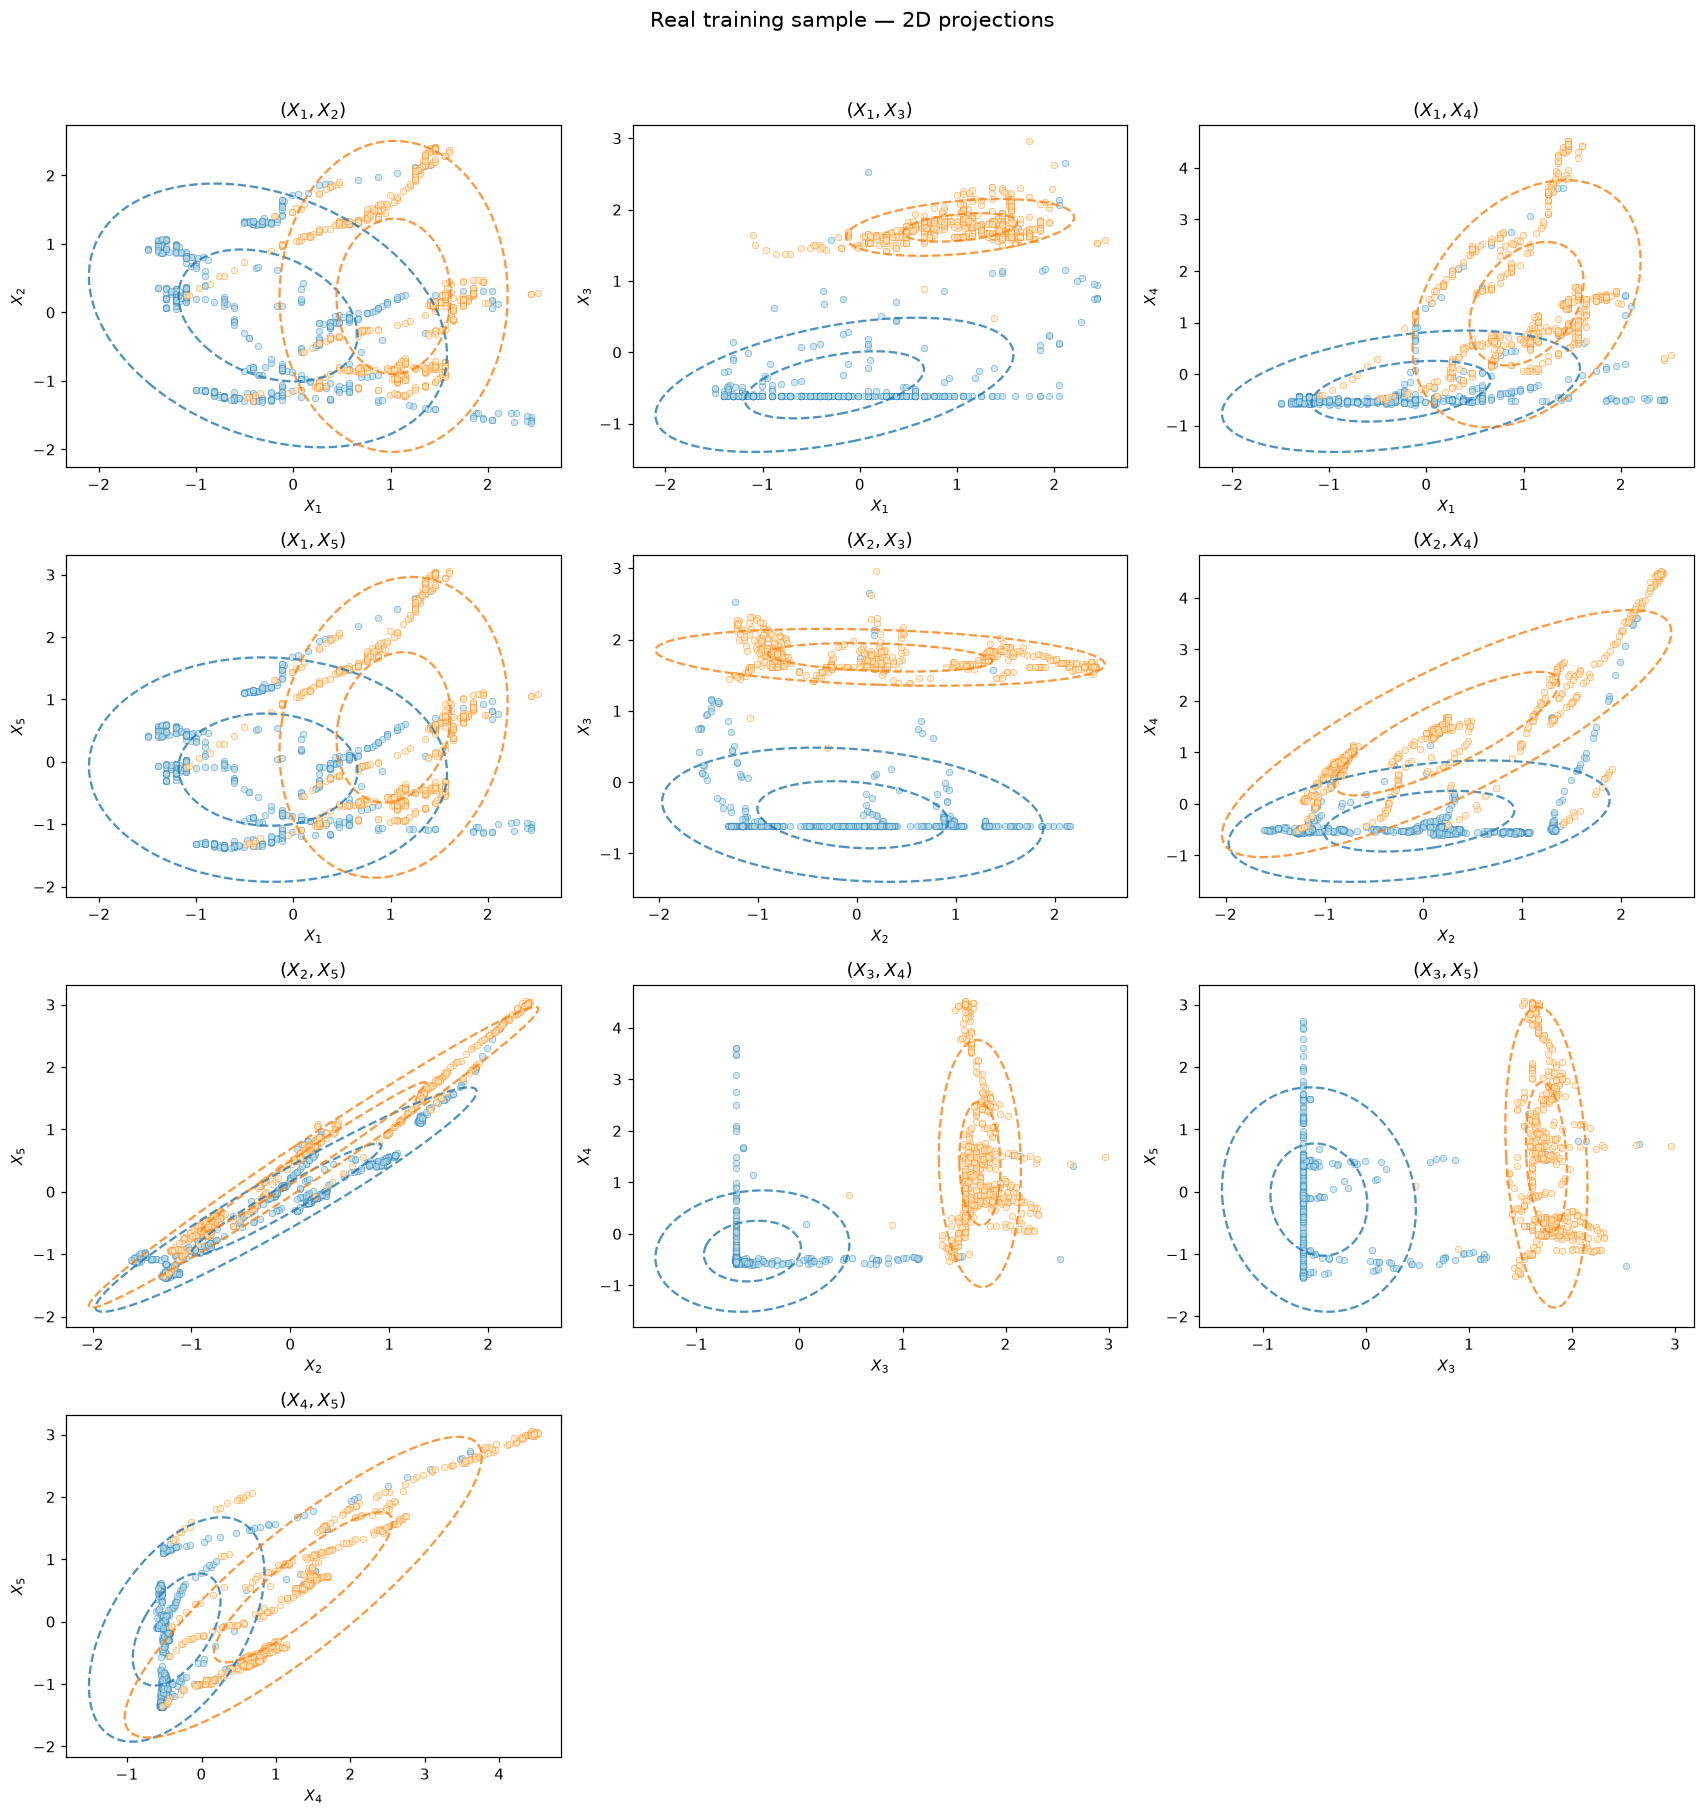
\includegraphics[width=\textwidth,height=0.80\textheight,keepaspectratio]{figures/geometry/occupancy/viz_2d_real_full_000002.png}
    \subcaption{Dados reais: concentração irregular e afastamento de uma geometria elíptica simples}
  \end{minipage}
  \sourcebelow{relatório publicado do cenário Occupancy Detection 000002}
\end{figure}

\begin{figure}[H]
  \ContinuedFloat
  \centering
  \caption[]{Comparação geométrica entre os dados reais de treinamento e as amostras sintéticas do Occupancy Detection (continuação)}
  \begin{minipage}{\textwidth}
    \centering
    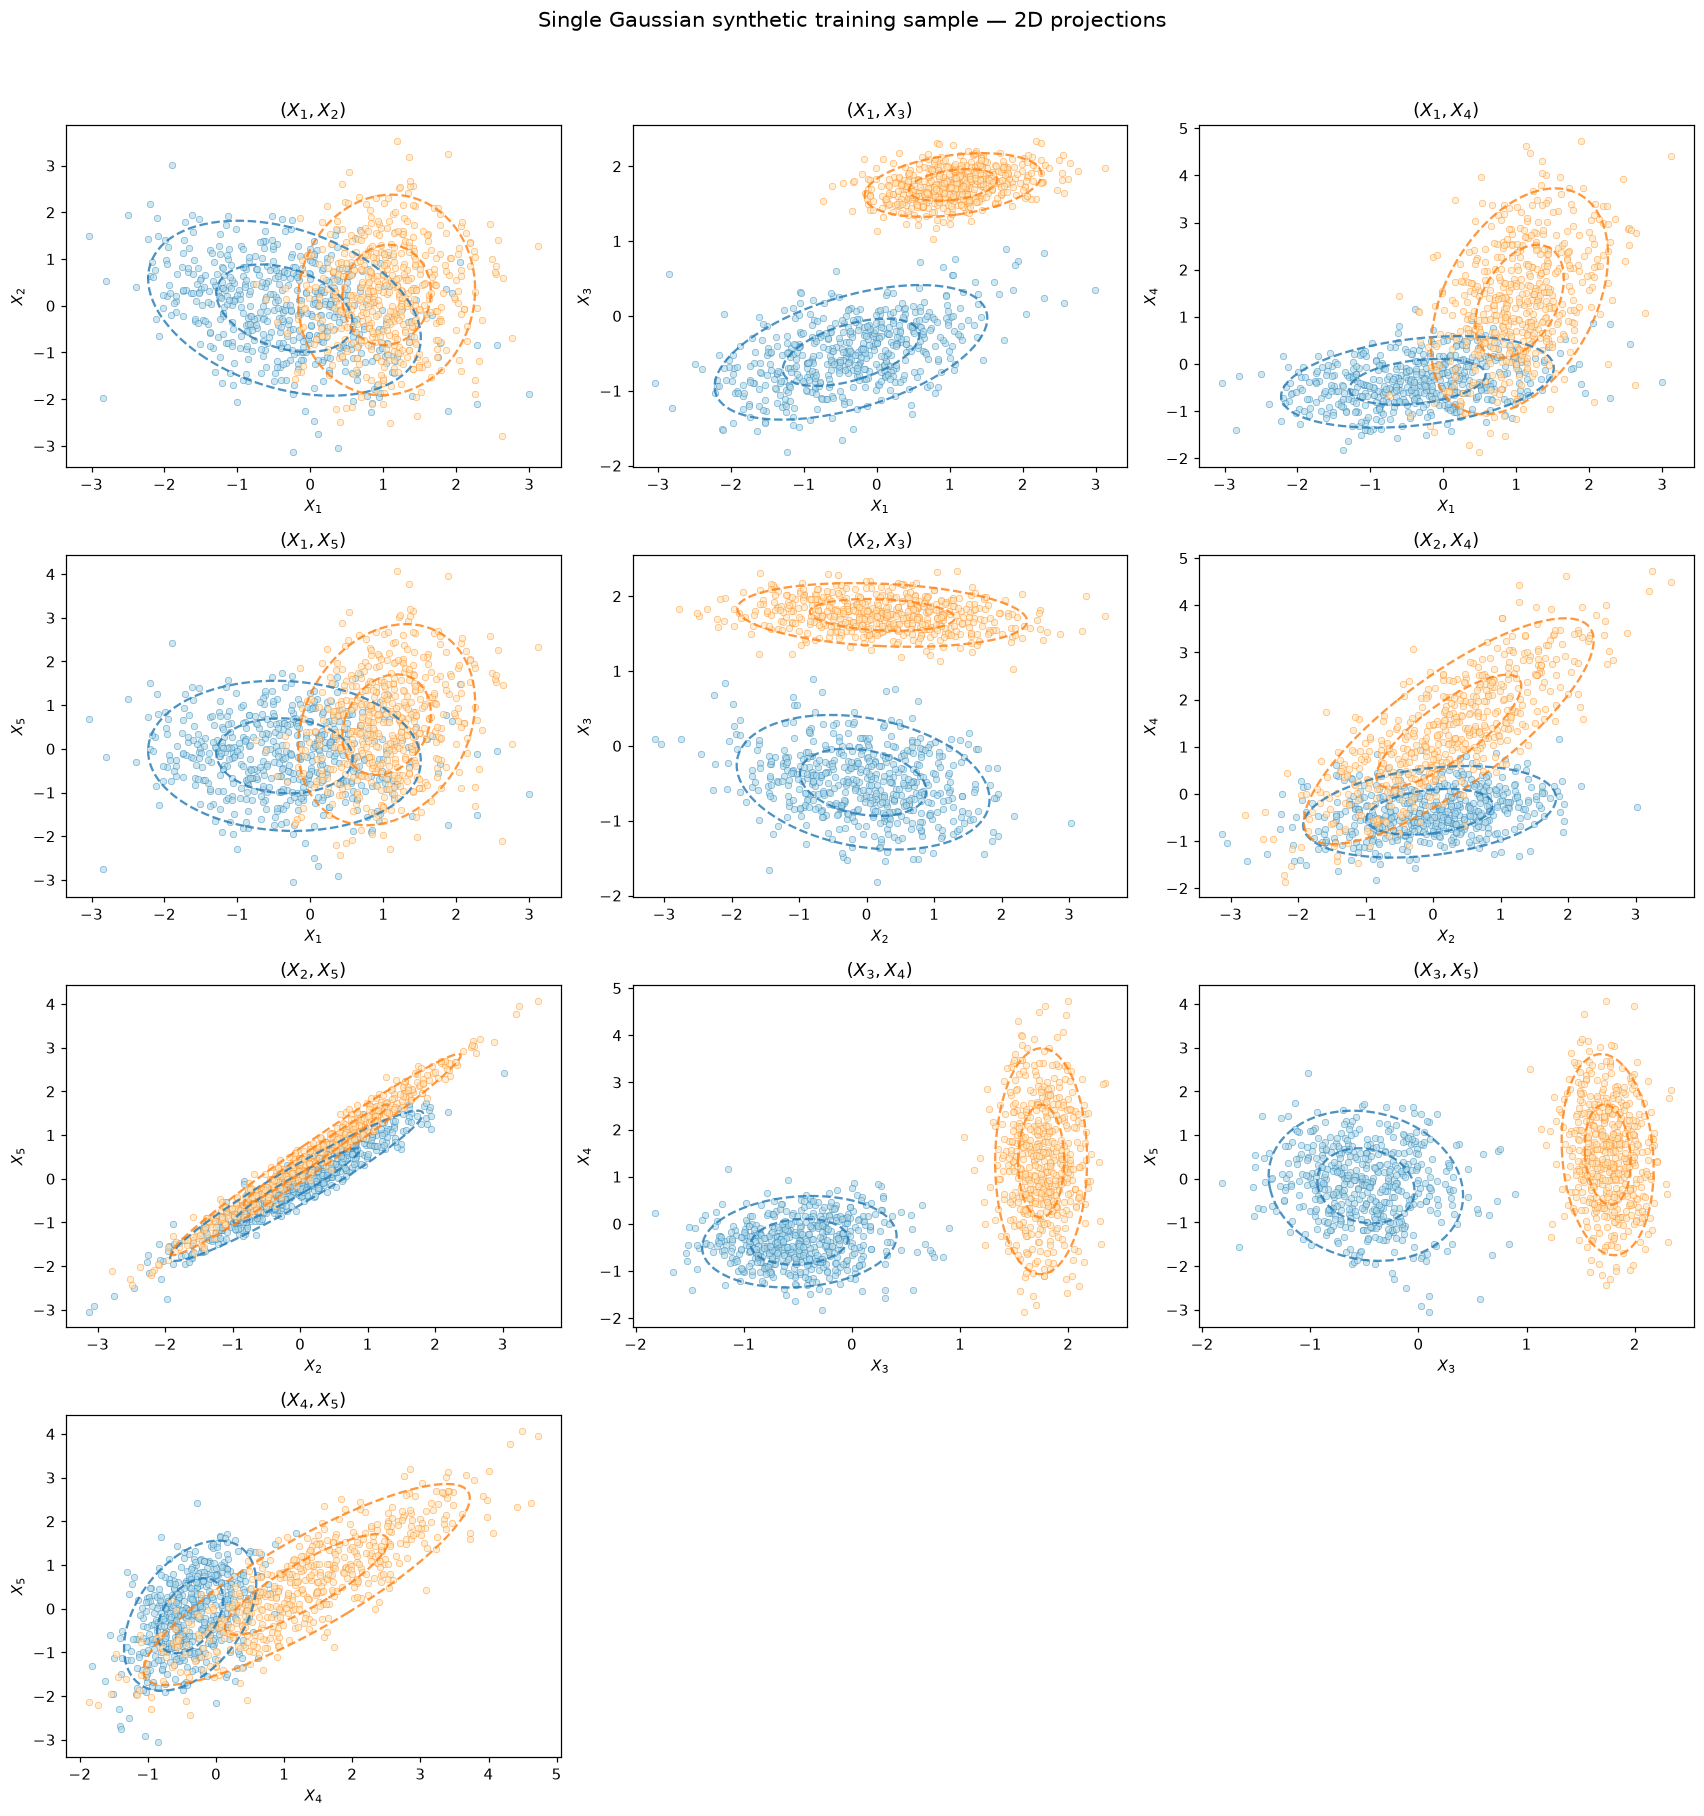
\includegraphics[width=\textwidth,height=0.80\textheight,keepaspectratio]{figures/geometry/occupancy/viz_2d_gaussian_full_000002.png}
    \subcaption{Gaussiana única: a aproximação regulariza fortemente as formas observadas}
  \end{minipage}
  \sourcebelow{relatório publicado do cenário Occupancy Detection 000002}
\end{figure}

\begin{figure}[H]
  \ContinuedFloat
  \centering
  \caption[]{Comparação geométrica entre os dados reais de treinamento e as amostras sintéticas do Occupancy Detection (continuação)}
  \begin{minipage}{\textwidth}
    \centering
    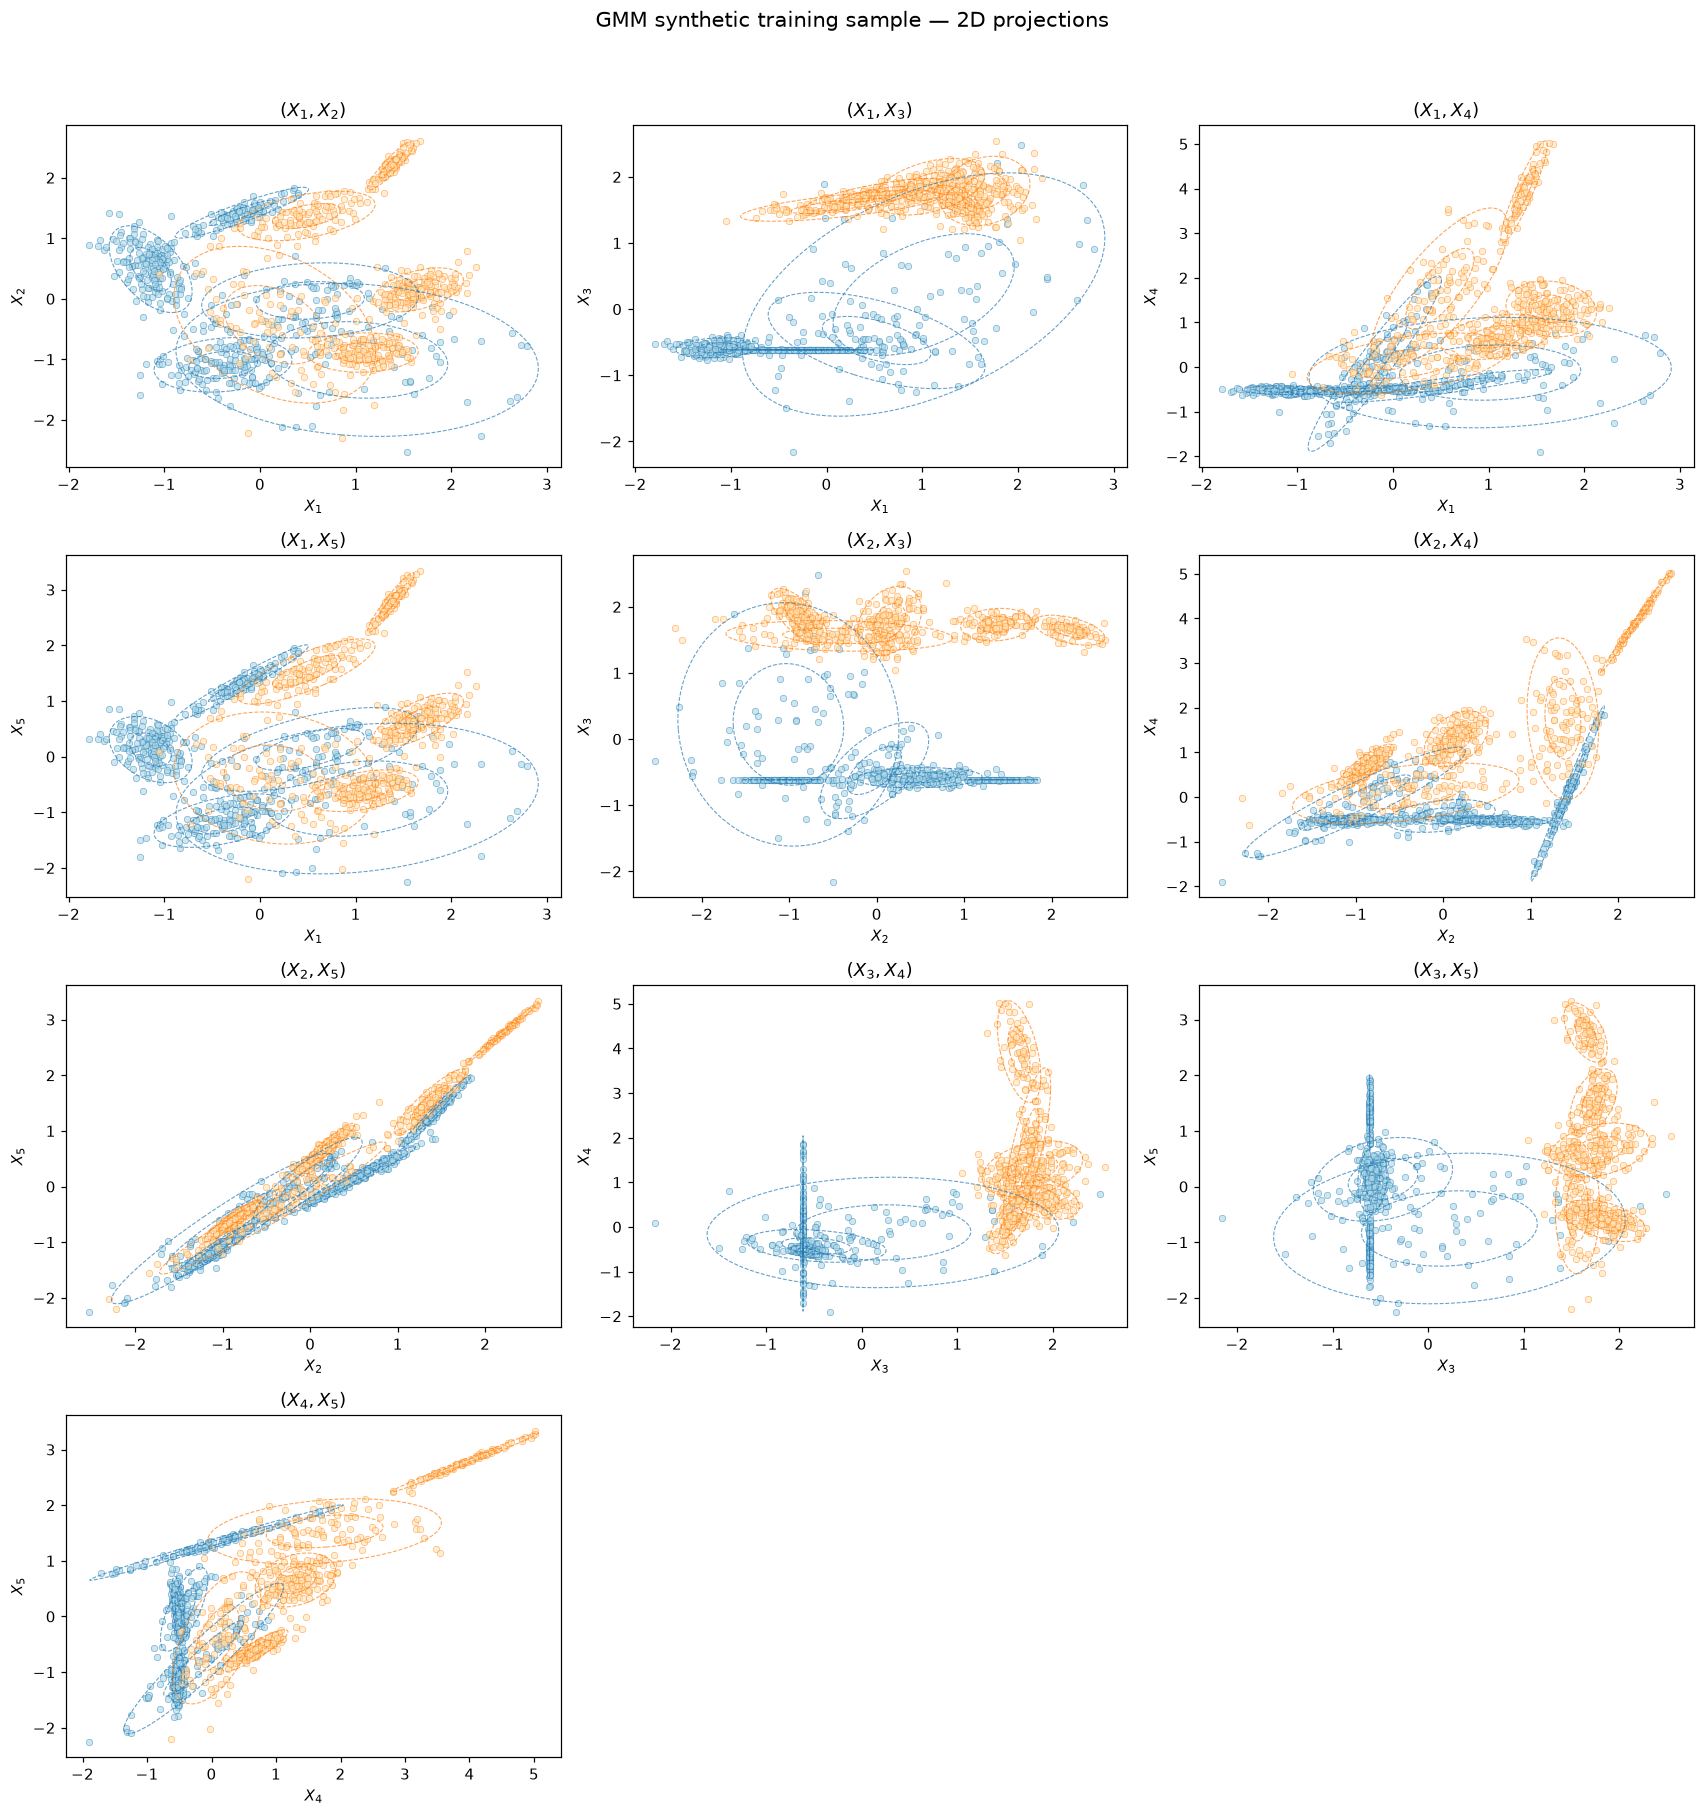
\includegraphics[width=\textwidth,height=0.80\textheight,keepaspectratio]{figures/geometry/occupancy/viz_2d_gmm_full_000002.png}
    \subcaption{GMM: a mistura acompanha melhor a forma empírica}
  \end{minipage}
  \sourcebelow{relatório publicado do cenário Occupancy Detection 000002}
  \notailustracao{A fidelidade geométrica é uma inspeção descritiva e não substitui os indicadores de preservação do perfil}
\end{figure}

\subsection{Ordenação global e relações efetivas de vencedor}

A Tabela~\ref{tab:occupancy-final} apresenta $\rankrho$ e $\AW$ no maior $n$ publicado anteriormente ($n=512$), herdados das versões anteriores deste relatório nos termos da nota da Seção~\ref{sec:resultados-guia}; $\AR$ e $\SR$ não puderam ser recalculados localmente e são reportados como indisponíveis. Para o SVM linear, o treinamento com amostras da Gaussiana única reproduziu melhor o ranking e as relações efetivas de vencedor do que o treinamento com amostras do GMM: $\rankrho=0{,}9528$ contra $0{,}8774$ e $\AW=0{,}9204$ contra $0{,}8624$. Isso ocorre apesar da inferioridade visual das amostras da Gaussiana única. Na regressão logística, o treinamento com amostras da Gaussiana única também apresentou correlação de ranking maior, enquanto aquele com amostras do GMM obteve \WinnersAgreement{} ligeiramente superior. No Gaussian Naive Bayes, ambos os braços reproduziram quase integralmente ranking e relações par a par.

\begin{table}[H]
  \centering
  \caption{Ordenação global e relações efetivas de vencedor no Occupancy Detection em $n=512$ (valores herdados; ver nota da Seção~\ref{sec:resultados-guia})}
  \label{tab:occupancy-final}
  \begin{adjustbox}{max width=\textwidth}
  \begin{tabular}{llSSl}
    \toprule
    Classificador & Braço de comparação & {$\rankrho$} & {$\AW$} & {$\AR$ / $\SR$} \\
    \midrule
    Linear SVM & Gaussiana única $\rightarrow$ Real & 0.9528 & 0.9204 & indisponível \\
    Linear SVM & GMM $\rightarrow$ Real             & 0.8774 & 0.8624 & indisponível \\
    Regressão Logística & Gaussiana única $\rightarrow$ Real & 0.9036 & 0.8839 & indisponível \\
    Regressão Logística & GMM $\rightarrow$ Real             & 0.8738 & 0.8903 & indisponível \\
    Gaussian Naive Bayes & Gaussiana única $\rightarrow$ Real & 0.9976 & 0.9892 & indisponível \\
    Gaussian Naive Bayes & GMM $\rightarrow$ Real             & 0.9996 & 0.9978 & indisponível \\
    \bottomrule
  \end{tabular}
  \end{adjustbox}
  \sourcebelow{elaboração própria a partir do relatório publicado do cenário Occupancy Detection 000002; ver limitação na Seção~\ref{sec:resultados-guia}}
\end{table}

\begin{figure}[H]
  \centering
  \caption{Correlação dos rankings completos no Occupancy Detection em $n=512$}
  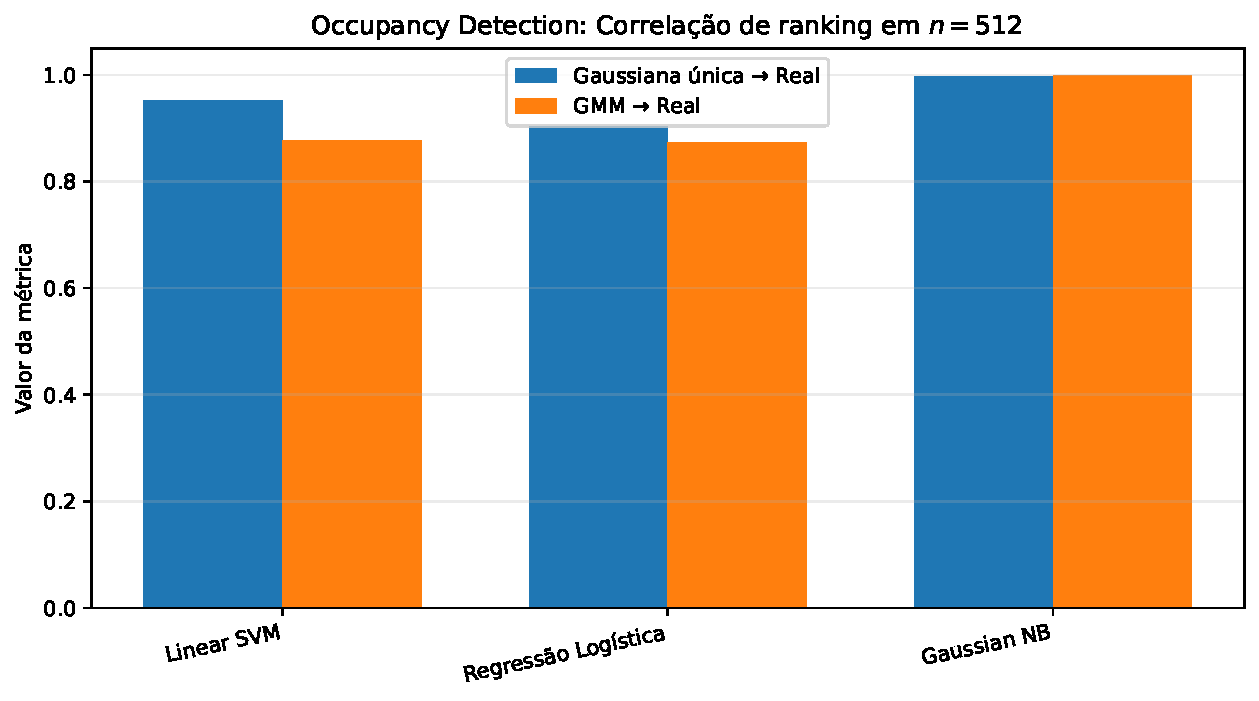
\includegraphics[width=0.87\textwidth]{figures/occupancy_ranking.pdf}
  \sourcebelow{elaboração própria a partir do relatório publicado do cenário Occupancy Detection 000002}
\end{figure}

\begin{figure}[H]
  \centering
  \caption{\WinnersAgreement{} no Occupancy Detection em $n=512$}
  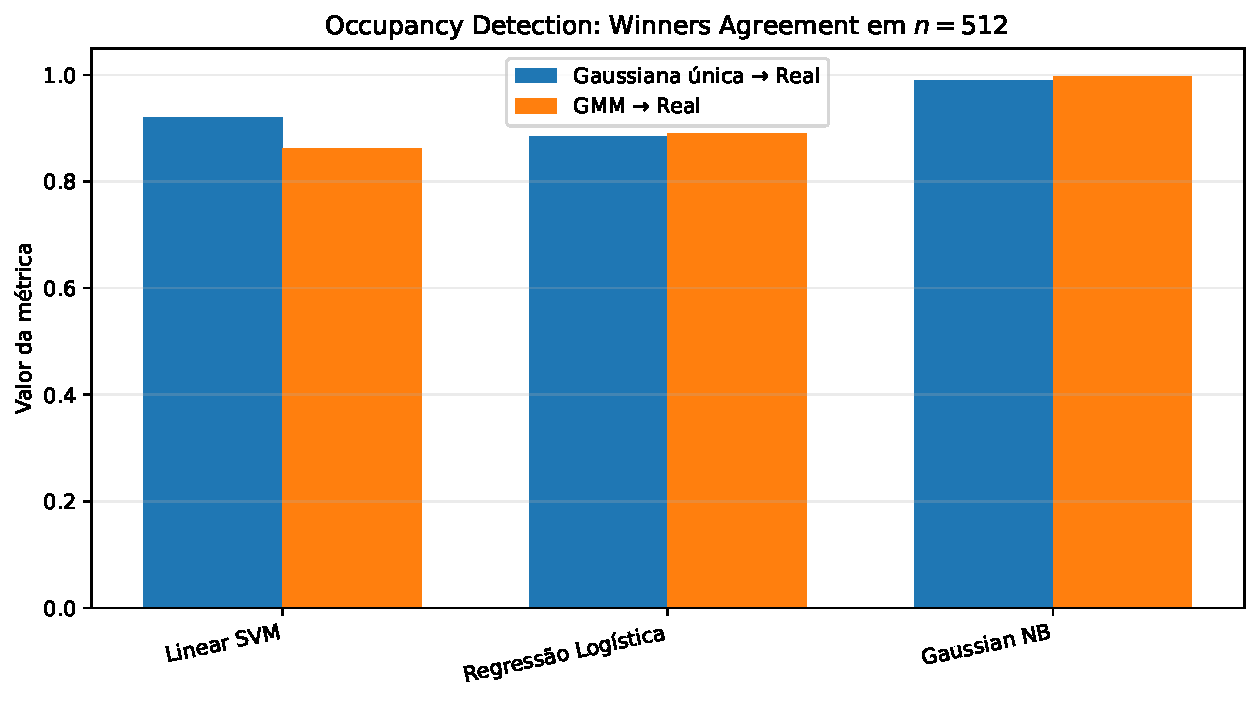
\includegraphics[width=0.87\textwidth]{figures/occupancy_winners.pdf}
  \sourcebelow{elaboração própria a partir do relatório publicado do cenário Occupancy Detection 000002}
\end{figure}

Os rankings de topo ajudam a interpretar essas métricas sem reduzir a análise ao primeiro colocado. No SVM linear do braço real, $\{X_1,X_3\}$ foi o melhor subconjunto, com perda $0{,}0107$. No braço treinado com amostras do GMM, esse par também ficou em primeiro lugar, com perda $0{,}0120$. No braço treinado com amostras da Gaussiana única, o par caiu para a quinta posição e $\{X_1,X_2,X_3,X_4\}$ ocupou o topo, embora a ordenação global tenha ficado mais próxima da referência do que aquela obtida com o GMM. O exemplo mostra por que coincidência do primeiro colocado e correlação de ranking não são equivalentes.

\subsection{Evolução do resultado par a par observado}

A Figura~\ref{fig:occupancy-winner-matrices} usa o resultado par a par observado do braço \RealToReal{} com SVM linear --- objeto que independe do esquema de métricas revisado nesta edição, pois corresponde diretamente à comparação $U_{ij}(n)$ definida na Equação~\eqref{eq:observed-outcome} --- para mostrar como as relações se reorganizam entre $n=2$ e $n=512$. No início da grade, subconjuntos de baixa cardinalidade vencem muitas comparações porque os modelos maiores sofrem maior variância de estimação; em $n=512$, a organização é mais estável e as combinações informativas passam a vencer uma parcela maior dos pares.

\begin{figure}[H]
  \centering
  \caption{Resultado par a par observado no Occupancy Detection, \RealToReal{}, SVM linear}
  \label{fig:occupancy-winner-matrices}
  \begin{minipage}[t]{0.47\textwidth}
    \centering
    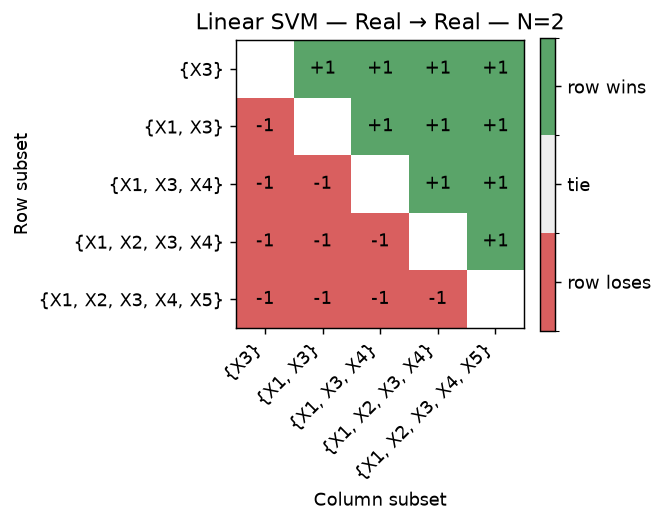
\includegraphics[width=\linewidth]{figures/winners/occupancy/graph_structural_winner_linear_svm_real_to_real_n2_full_000002.png}
    \subcaption{$n=2$}
  \end{minipage}
  \hfill
  \begin{minipage}[t]{0.47\textwidth}
    \centering
    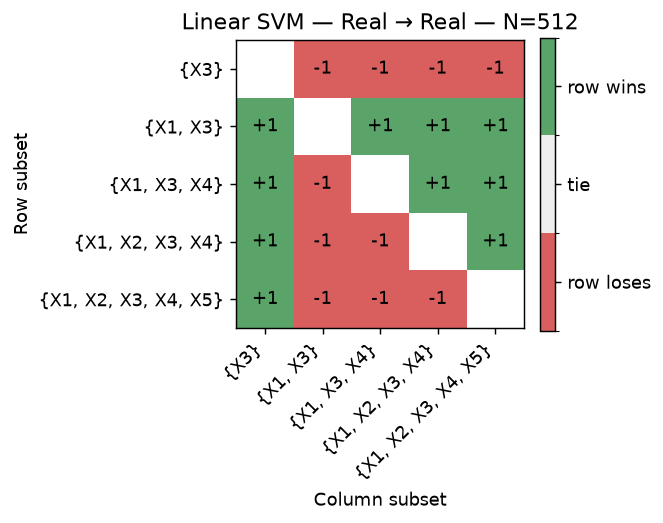
\includegraphics[width=\linewidth]{figures/winners/occupancy/graph_structural_winner_linear_svm_real_to_real_n512_full_000002.png}
    \subcaption{$n=512$}
  \end{minipage}
  \sourcebelow{relatório publicado do cenário Occupancy Detection 000002}
  \notailustracao{A implementação numérica usa apenas os pares não ordenados da região triangular. A matriz quadrada é uma visualização redundante: a diagonal não se aplica e cada célula indica se o subconjunto da linha vence, perde ou está indefinido contra o da coluna. Os painéis publicados exibem os melhores subconjuntos de cada cardinalidade}
\end{figure}

\subsection{Existência e tamanho amostral das inversões}

$\AR$, $\DR$ e $\SR$ para o Occupancy Detection não puderam ser recalculados nesta revisão pela ausência local dos resultados brutos da execução \textit{full} do cenário 000002 (Seção~\ref{sec:resultados-guia}). As figuras de matriz de inversões e as curvas de $\NstarHistorical$ anteriormente publicadas para este cenário dependiam do objeto retirado do arcabouço ativo e não são reproduzidas aqui. A leitura qualitativa preservável --- de que a ordenação e as relações efetivas de vencedor foram bem preservadas no Gaussian Naive Bayes e de forma mais heterogênea nos classificadores lineares --- permanece válida, mas não pode ser complementada, nesta revisão, por uma leitura numérica da existência ou do regime amostral das inversões.

\section{UCI Air Quality}

\subsection{Geometria e referência real}

As projeções do Air Quality são mais compatíveis com regiões gaussianas do que as do Occupancy. Embora existam assimetrias, correlações fortes, sensibilidade cruzada e deriva temporal, as classes formam regiões mais regulares no espaço padronizado. A Gaussiana única e o GMM reproduzem visualmente uma parcela maior da organização real, sobretudo nos pares de sensores mais correlacionados com a referência de benzeno, como mostra a Figura~\ref{fig:geom-air-resultados}.

\begin{figure}[H]
  \centering
  \caption{Comparação geométrica entre os dados reais de treinamento e as amostras sintéticas do UCI Air Quality}
  \label{fig:geom-air-resultados}
  \begin{minipage}{\textwidth}
    \centering
    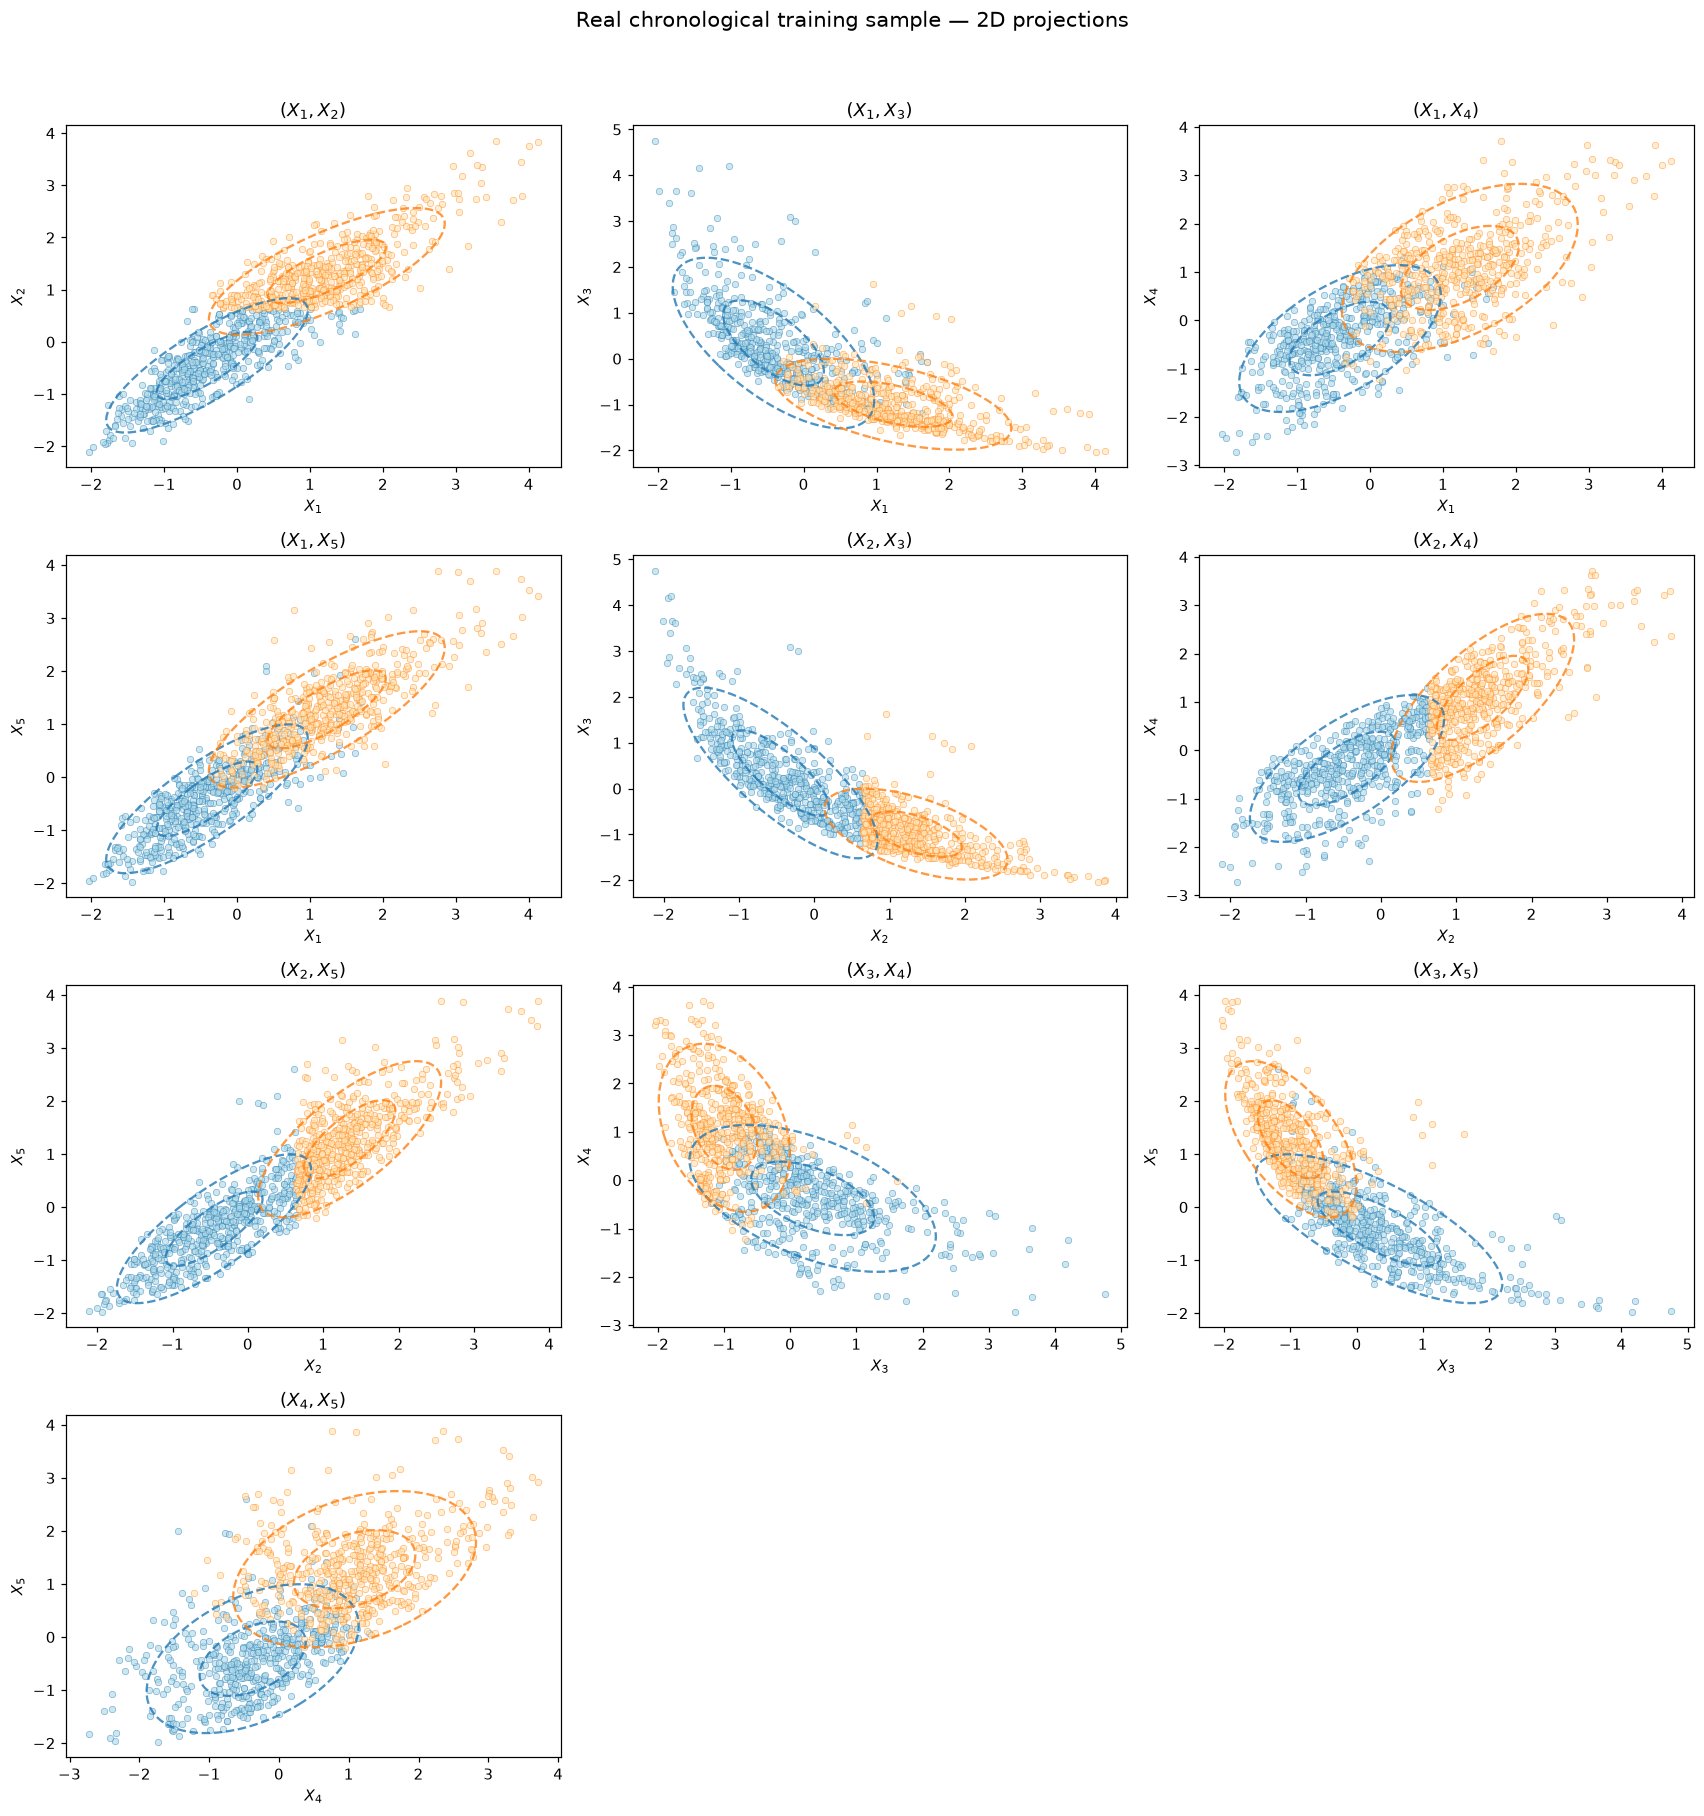
\includegraphics[width=\textwidth,height=0.80\textheight,keepaspectratio]{figures/geometry/air_quality/viz_2d_real_full_000005.png}
    \subcaption{Dados reais}
  \end{minipage}
  \sourcebelow{relatório publicado do cenário Air Quality 000005}
\end{figure}

\begin{figure}[H]
  \ContinuedFloat
  \centering
  \caption[]{Comparação geométrica entre os dados reais de treinamento e as amostras sintéticas do UCI Air Quality (continuação)}
  \begin{minipage}{\textwidth}
    \centering
    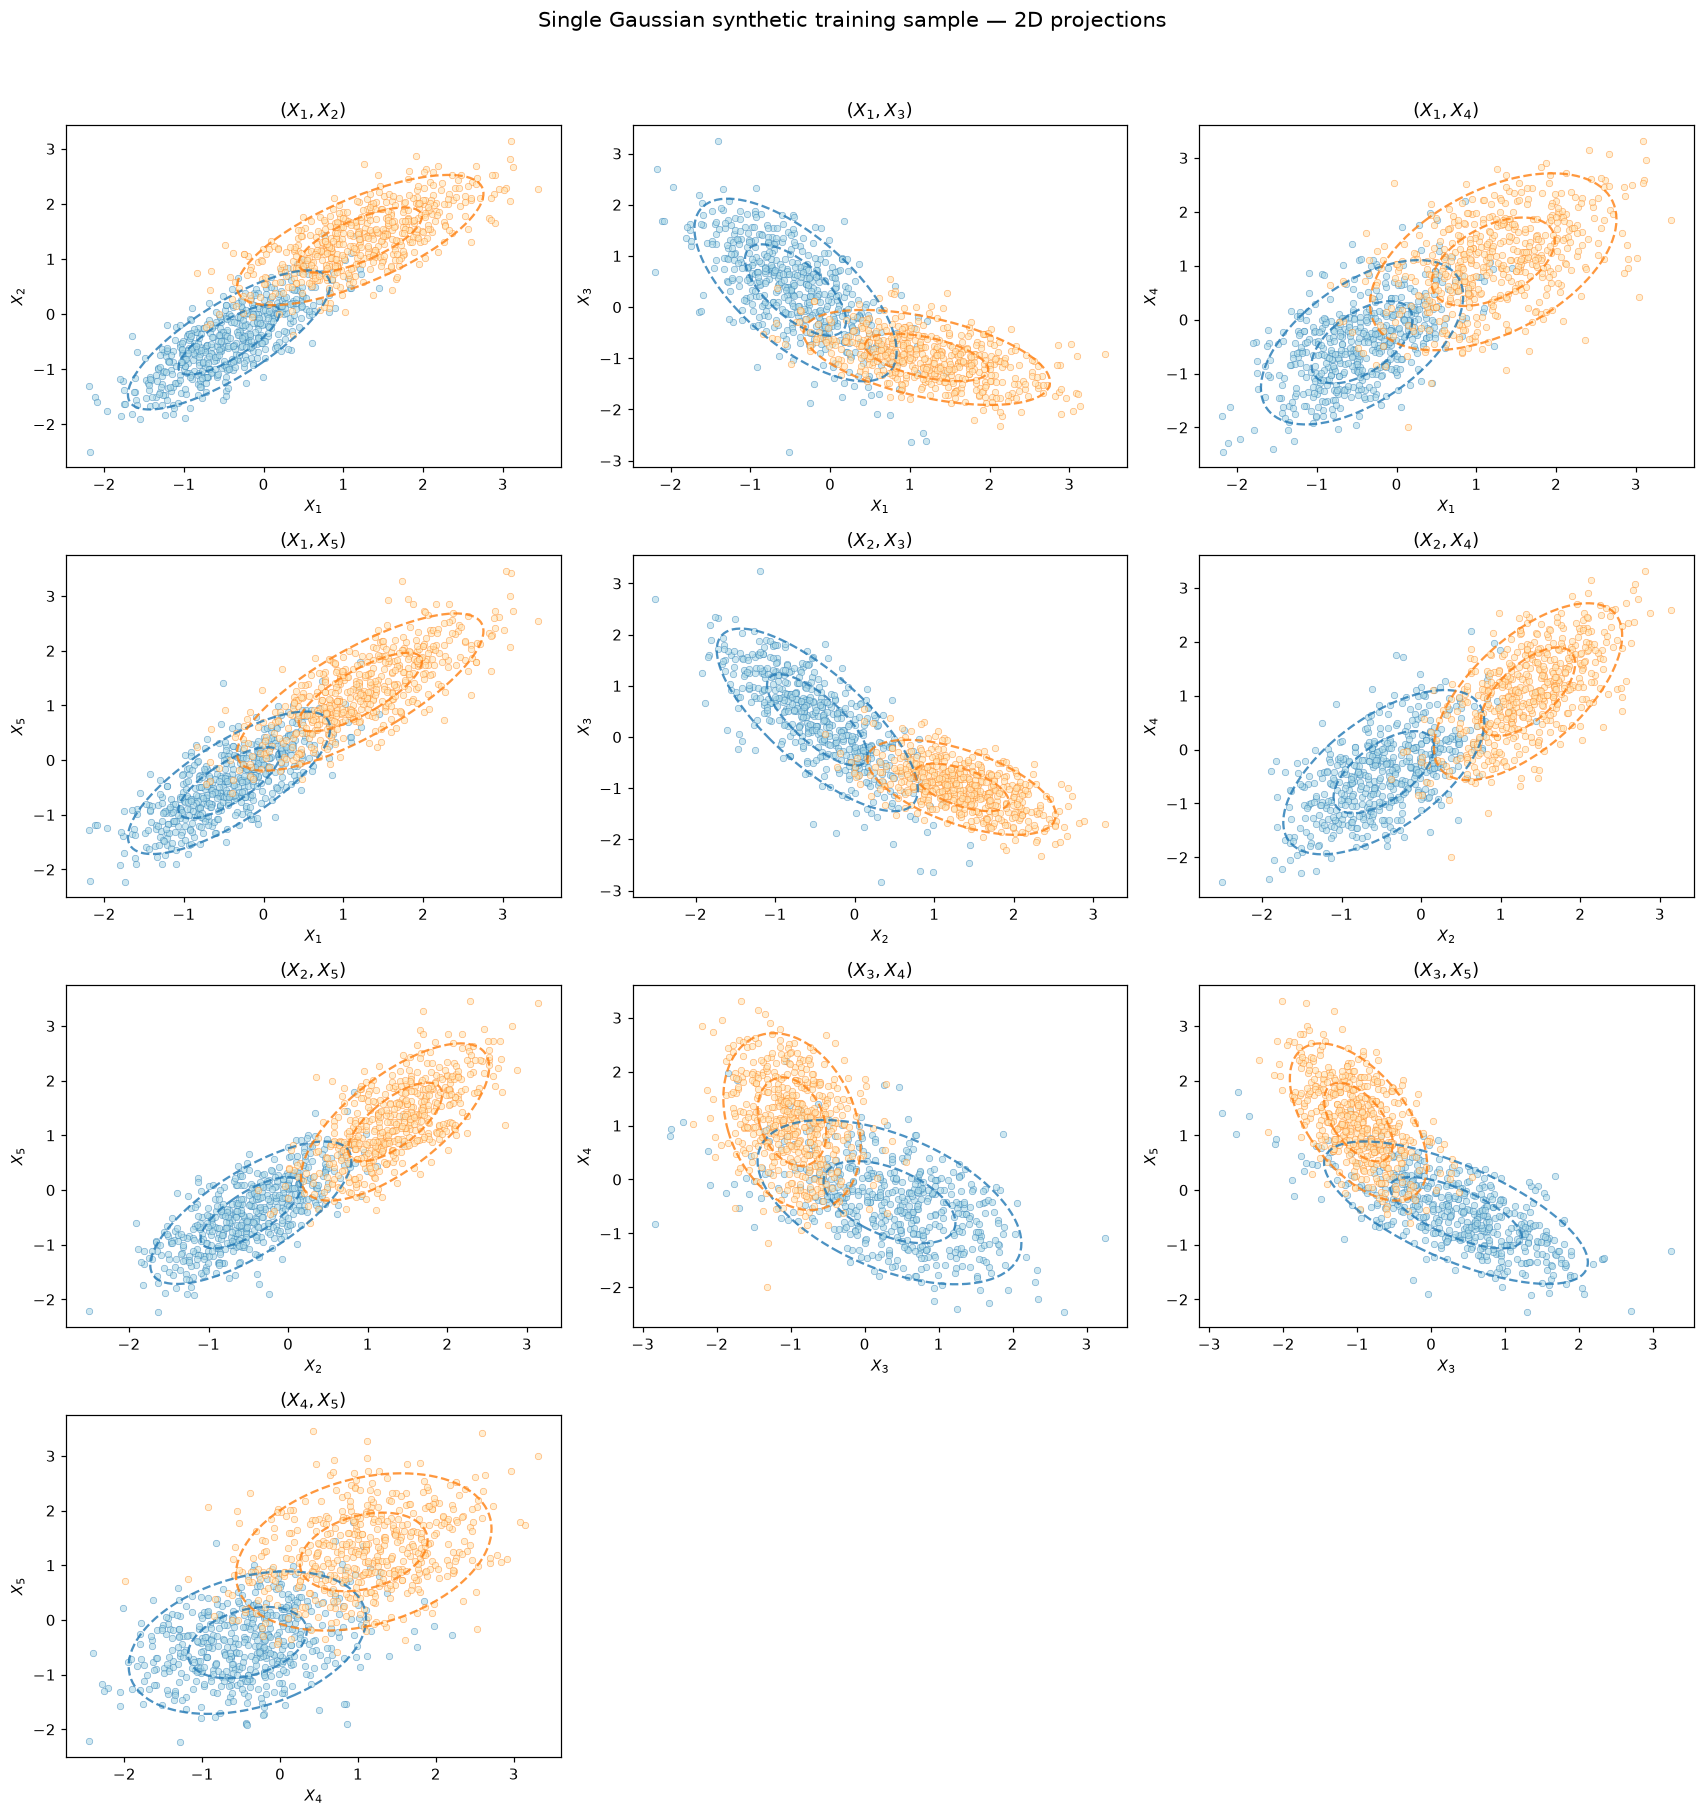
\includegraphics[width=\textwidth,height=0.80\textheight,keepaspectratio]{figures/geometry/air_quality/viz_2d_gaussian_full_000005.png}
    \subcaption{Gaussiana única}
  \end{minipage}
  \sourcebelow{relatório publicado do cenário Air Quality 000005}
\end{figure}

\begin{figure}[H]
  \ContinuedFloat
  \centering
  \caption[]{Comparação geométrica entre os dados reais de treinamento e as amostras sintéticas do UCI Air Quality (continuação)}
  \begin{minipage}{\textwidth}
    \centering
    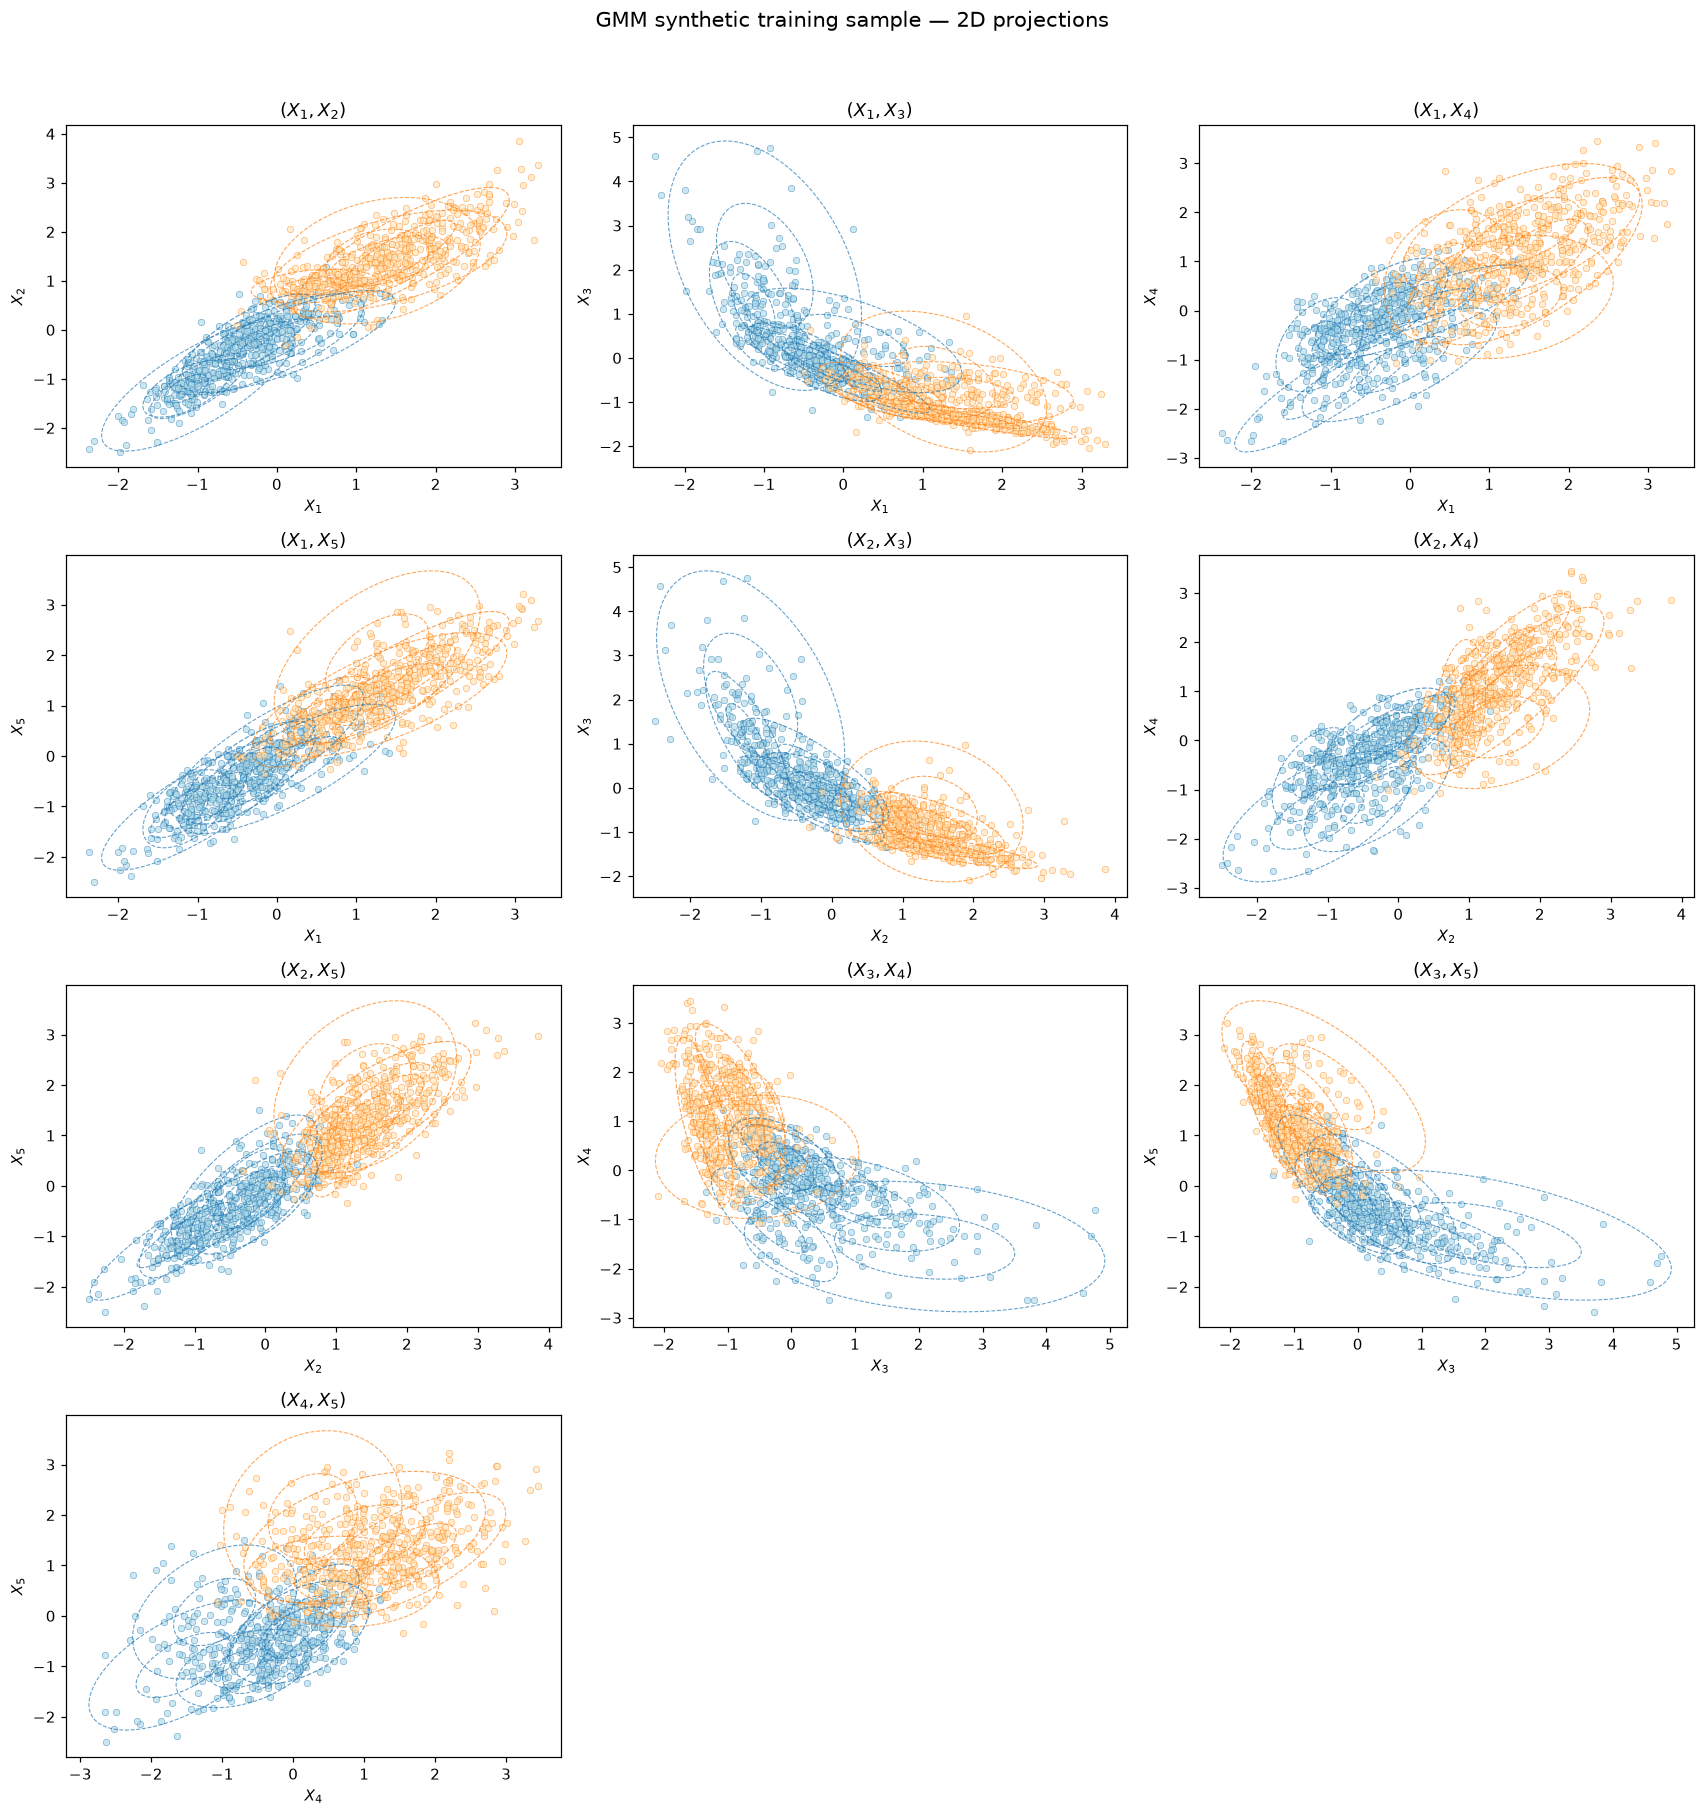
\includegraphics[width=\textwidth,height=0.80\textheight,keepaspectratio]{figures/geometry/air_quality/viz_2d_gmm_full_000005.png}
    \subcaption{GMM}
  \end{minipage}
  \sourcebelow{relatório publicado do cenário Air Quality 000005}
\end{figure}

\subsection{Ordenação global e relações efetivas de vencedor}

A Tabela~\ref{tab:air-final} mostra uma preservação elevada do ranking e das relações efetivas de vencedor para todos os classificadores, nos mesmos termos herdados descritos na Seção~\ref{sec:resultados-guia}. O treinamento com amostras do GMM superou aquele com amostras da Gaussiana única para SVM e regressão logística em ambos os indicadores disponíveis. O resultado mais forte ocorreu com Gaussian Naive Bayes: o braço da Gaussiana única alcançou $\rankrho=1$ e $\AW=1$, enquanto o braço do GMM alcançou $0{,}9996$ e $0{,}9978$.

\begin{table}[H]
  \centering
  \caption{Ordenação global e relações efetivas de vencedor no UCI Air Quality em $n=512$ (valores herdados; ver nota da Seção~\ref{sec:resultados-guia})}
  \label{tab:air-final}
  \begin{adjustbox}{max width=\textwidth}
  \begin{tabular}{llSSl}
    \toprule
    Classificador & Braço de comparação & {$\rankrho$} & {$\AW$} & {$\AR$ / $\SR$} \\
    \midrule
    Linear SVM & Gaussiana única $\rightarrow$ Real & 0.8944 & 0.8882 & indisponível \\
    Linear SVM & GMM $\rightarrow$ Real             & 0.9580 & 0.9333 & indisponível \\
    Regressão Logística & Gaussiana única $\rightarrow$ Real & 0.9359 & 0.9118 & indisponível \\
    Regressão Logística & GMM $\rightarrow$ Real             & 0.9839 & 0.9613 & indisponível \\
    Gaussian Naive Bayes & Gaussiana única $\rightarrow$ Real & 1.0000 & 1.0000 & indisponível \\
    Gaussian Naive Bayes & GMM $\rightarrow$ Real             & 0.9996 & 0.9978 & indisponível \\
    \bottomrule
  \end{tabular}
  \end{adjustbox}
  \sourcebelow{elaboração própria a partir do relatório publicado do cenário Air Quality 000005; ver limitação na Seção~\ref{sec:resultados-guia}}
\end{table}

\begin{figure}[H]
  \centering
  \caption{Correlação dos rankings completos no UCI Air Quality em $n=512$}
  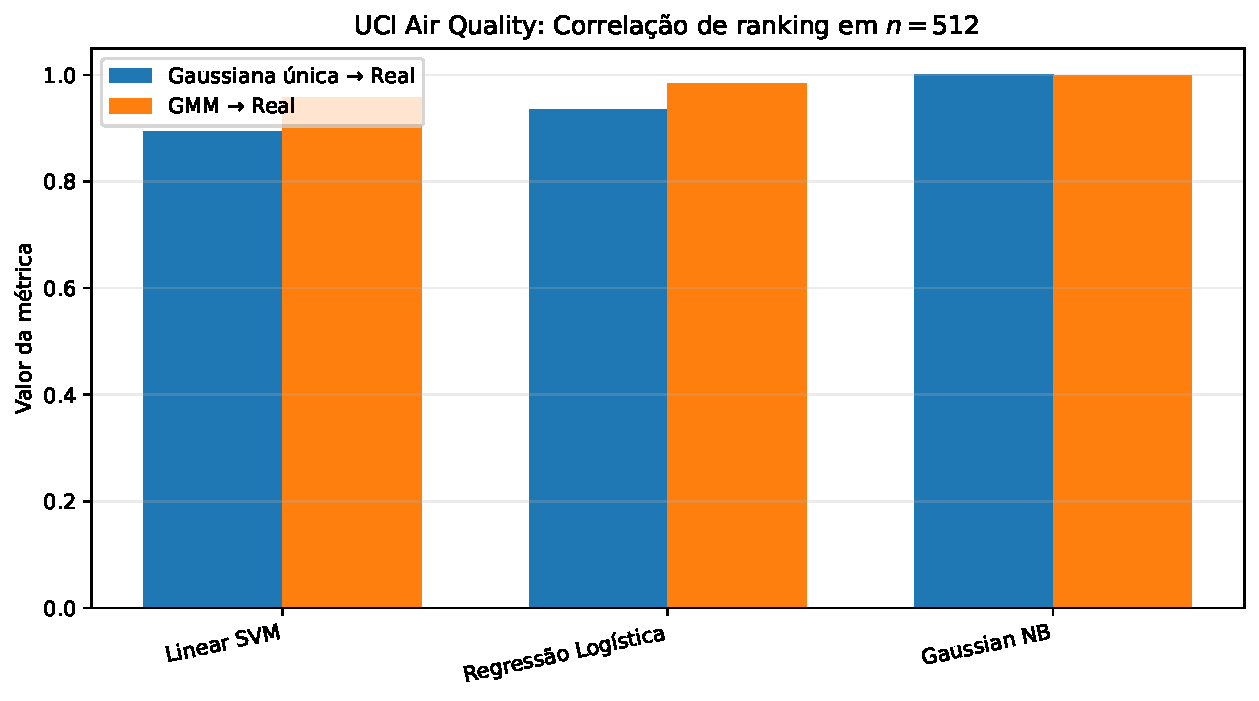
\includegraphics[width=0.87\textwidth]{figures/air_quality_ranking.pdf}
  \sourcebelow{elaboração própria a partir do relatório publicado do cenário Air Quality 000005}
\end{figure}

\begin{figure}[H]
  \centering
  \caption{\WinnersAgreement{} no UCI Air Quality em $n=512$}
  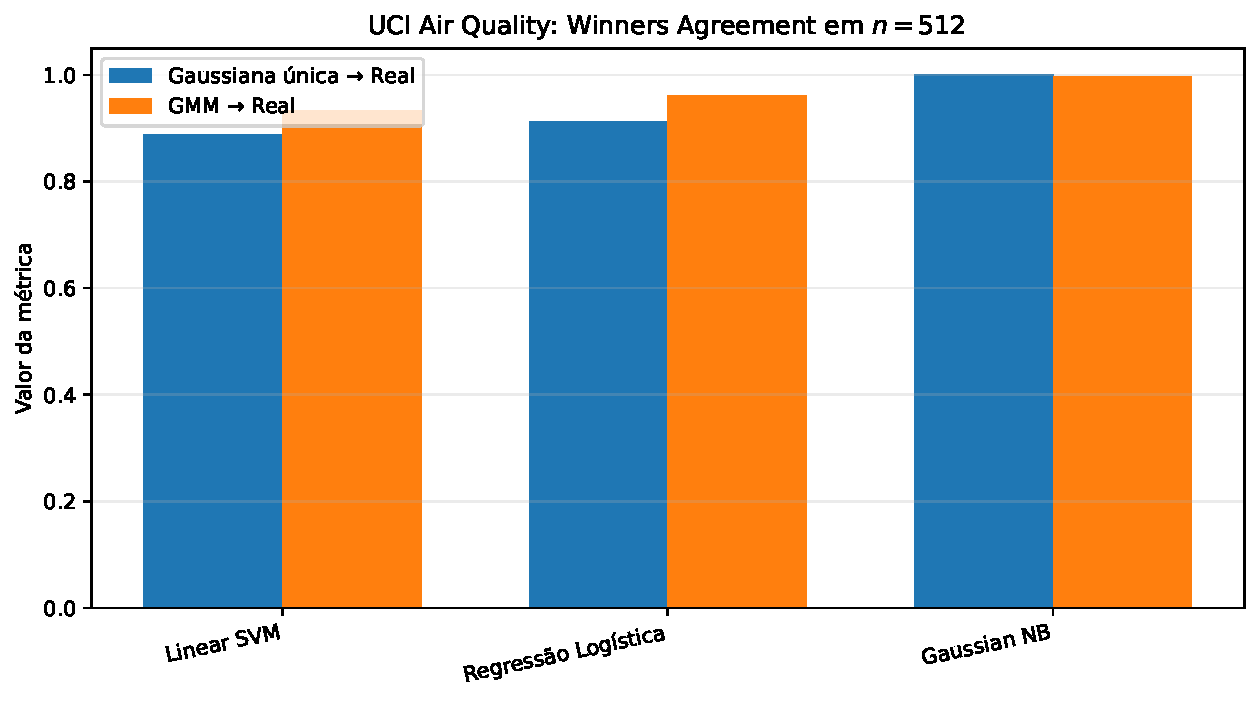
\includegraphics[width=0.87\textwidth]{figures/air_quality_winners.pdf}
  \sourcebelow{elaboração própria a partir do relatório publicado do cenário Air Quality 000005}
\end{figure}

A combinação Air Quality--Gaussian Naive Bayes permanece a evidência mais clara, entre os indicadores disponíveis nesta revisão, de preservação quase integral da ordenação global e das relações efetivas de vencedor. A existência e o regime amostral das inversões para esse par dataset--classificador não puderam ser recalculados nesta revisão (Seção~\ref{sec:resultados-guia}) e não são, portanto, comparados aqui ao exemplo do SUPPORT2 apresentado na Seção~\ref{sec:support2-rf}.

\section{SUPPORT2}

\subsection{Ordenação global e relações efetivas de vencedor com classificadores lineares e Gaussian Naive Bayes}

O SUPPORT2 amplia o problema para sete canais e 127 subconjuntos. A Tabela~\ref{tab:support2-original} resume o cenário 000007 (execução \textit{full}, $n\leq512$), nos mesmos termos herdados da Seção~\ref{sec:resultados-guia}. Ranking e relações efetivas de vencedor permaneceram elevados em várias configurações, particularmente no SVM com GMM e na regressão logística.

\begin{table}[H]
  \centering
  \caption{Ordenação global e relações efetivas de vencedor no SUPPORT2, cenário 000007, em $n=512$ (valores herdados; ver nota da Seção~\ref{sec:resultados-guia})}
  \label{tab:support2-original}
  \begin{adjustbox}{max width=\textwidth}
  \begin{tabular}{llSSl}
    \toprule
    Classificador & Braço de comparação & {$\rankrho$} & {$\AW$} & {$\AR$ / $\SR$} \\
    \midrule
    Linear SVM & Gaussiana única $\rightarrow$ Real & 0.8672 & 0.8614 & indisponível \\
    Linear SVM & GMM $\rightarrow$ Real             & 0.9708 & 0.9344 & indisponível \\
    Regressão Logística & Gaussiana única $\rightarrow$ Real & 0.9853 & 0.9514 & indisponível \\
    Regressão Logística & GMM $\rightarrow$ Real             & 0.9827 & 0.9461 & indisponível \\
    Gaussian Naive Bayes & Gaussiana única $\rightarrow$ Real & 0.7915 & 0.7951 & indisponível \\
    Gaussian Naive Bayes & GMM $\rightarrow$ Real             & 0.9144 & 0.8715 & indisponível \\
    \bottomrule
  \end{tabular}
  \end{adjustbox}
  \sourcebelow{elaboração própria a partir do relatório publicado do cenário SUPPORT2 000007; ver limitação na Seção~\ref{sec:resultados-guia}}
\end{table}

\subsection{Random Forest: desempenho absoluto e preservação do perfil}
\label{sec:support2-rf}

O cenário 000008 (execução \textit{full}, $n\leq512$) executou somente Random Forest, com a mesma grade, os mesmos 127 subconjuntos e o mesmo teste real fixo. No maior $n$ publicado, a menor perda de cada braço permaneceu próxima de $0{,}455$. Como a classe minoritária representa 832 das 1.775 observações de teste, o erro de um classificador que sempre prediz a classe majoritária é aproximadamente $0{,}4687$. O ganho absoluto do melhor Random Forest sobre esse referencial é, portanto, pequeno.

\begin{figure}[H]
  \centering
  \caption{Menor perda do Random Forest no SUPPORT2 em $n=512$ (execução \textit{full}, cenário 000008)}
  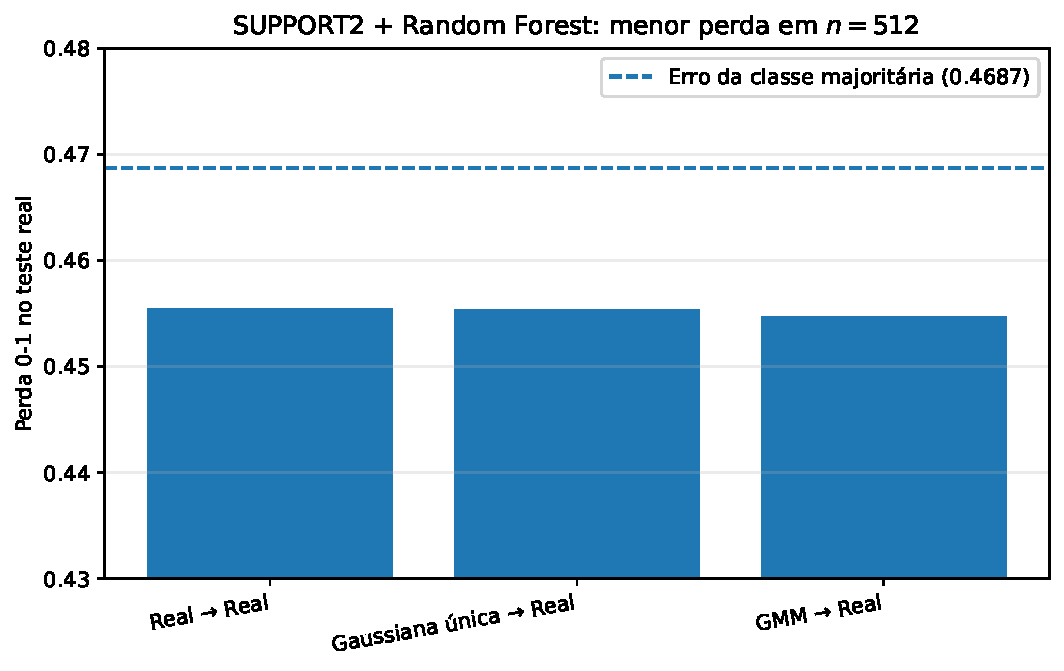
\includegraphics[width=0.80\textwidth]{figures/support2_rf_best_losses.pdf}
  \sourcebelow{elaboração própria a partir do relatório publicado do cenário SUPPORT2 000008}
  \notailustracao{A linha tracejada representa o erro de classificação obtido ao predizer sempre a classe majoritária no teste real. Este valor de perda não depende do esquema de métricas revisado e é reportado sem a ressalva de disponibilidade da Seção~\ref{sec:resultados-guia}}
\end{figure}

$\rankrho$ e $\AW$ herdados do cenário 000008 mostram que esse baixo desempenho absoluto não impediu preservação elevada da ordenação e das relações efetivas de vencedor: o braço treinado com amostras da Gaussiana única atingiu $\rankrho=0{,}8387$ e $\AW=0{,}8282$; o braço treinado com amostras do GMM atingiu $0{,}8665$ e $0{,}8429$. $\AR$, $\DR$ e $\SR$ de escala completa ($n\leq512$) não puderam ser recalculados para este cenário (Seção~\ref{sec:resultados-guia}); as antigas figuras de matrizes dirigidas de $\NstarHistorical$ e de curvas cooperativas com marcação de último cruzamento, publicadas para este cenário, dependiam do objeto retirado do arcabouço ativo e não são reproduzidas.

\begin{keyresultbox}[Exemplo numérico corrente: SUPPORT2, execução \textit{smoke}]
Para oferecer ao menos um exemplo de $\AR$, $\DR$ e $\SR$ calculado diretamente pelo código atual sobre resultados brutos localmente persistidos, a Tabela~\ref{tab:support2-smoke} e a Figura~\ref{fig:wr-matrices-support2-cap7} usam a execução \textit{smoke} do SUPPORT2 (\texttt{scenario\_run\_id=0}, grade $n\in\{2,4,8,16,32\}$, sete subconjuntos de referência selecionados um por cardinalidade). Esta execução \textbf{não é comparável em escala} à execução \textit{full} discutida acima ($n\leq512$, 127 subconjuntos completos): ela serve apenas para demonstrar, com números genuínos, a leitura conjunta dos quatro indicadores, e não para substituir ou estender os resultados de escala completa publicados anteriormente.
\end{keyresultbox}

\begin{table}[H]
  \centering
  \caption{Indicadores de preservação do perfil no SUPPORT2, execução \textit{smoke} (\texttt{scenario\_run\_id=0}), $n_t\leq32$, recalculados diretamente pelo código atual}
  \label{tab:support2-smoke}
  \begin{adjustbox}{max width=\textwidth}
  \begin{tabular}{llSSSSl}
    \toprule
    Classificador & Braço & {$\rankrho$} & {$\AW$} & {$\AR$} & {$\SR$} & {Pares (ref./braço/compart./união)} \\
    \midrule
    Linear SVM & Gaussiana única $\rightarrow$ Real & 0.0105 & 0.5043 & 0.7280 & 0.7283 & 6651 / 6886 / 5703 / 7834 \\
    Linear SVM & GMM $\rightarrow$ Real             & 0.2712 & 0.5909 & 0.7937 & 0.6886 & 6651 / 7446 / 6238 / 7859 \\
    Random Forest & Gaussiana única $\rightarrow$ Real & 0.6236 & 0.7309 & 0.4790 & 0.8815 & 4826 / 5737 / 3421 / 7142 \\
    Random Forest & GMM $\rightarrow$ Real             & 0.5335 & 0.6869 & 0.4668 & 0.8787 & 4826 / 5629 / 3327 / 7128 \\
    \bottomrule
  \end{tabular}
  \end{adjustbox}
  \sourcebelow{recomputado diretamente dos resultados persistidos em \texttt{output/validation/support2-random-forest-smoke/}, usando \texttt{coinfosim.results.structural.scenario\_structural\_fidelity}; ver Apêndice~B para o comando exato}
  \notailustracao{$q=127$ subconjuntos; $q(q-1)/2=8001$ pares não ordenados totais em todas as linhas. $\DR$ (distância média em $\log_2$, não tabulada por espaço) foi de $1{,}087$ (SVM, Gaussiana) e $1{,}245$ (SVM, GMM) contra $0{,}474$ (RF, Gaussiana) e $0{,}485$ (RF, GMM) --- o Random Forest concentrou as inversões compartilhadas em regimes amostrais mais próximos entre braços, mesmo com $\AR$ mais baixo}
\end{table}

Nesta execução reduzida, o Random Forest preservou pior a \emph{existência} das inversões do que o SVM linear ($\AR\approx0{,}47$--$0{,}48$ contra $0{,}73$--$0{,}79$), mas, condicional aos pares que efetivamente invertem em ambos os braços, preservou melhor o \emph{regime amostral} dessas inversões ($\SR\approx0{,}88$ contra $0{,}69$--$0{,}73$). O SVM linear, por sua vez, teve ordenação global quase não preservada ($\rankrho$ próximo de zero) apesar de $\AW$ moderado --- um lembrete de que os quatro indicadores podem divergir fortemente mesmo em uma única execução. Esses achados são específicos da escala \textit{smoke} e não devem ser extrapolados para a escala completa sem regeneração dos dados brutos correspondentes.

\begin{figure}[H]
  \centering
  \caption{Matriz de vencedores $\mathbf{W}$ e matriz de inversões $\mathbf{R}$, SUPPORT2 \textit{smoke}, Random Forest, \RealToReal{} e \GaussianToReal{}}
  \label{fig:wr-matrices-support2-cap7}
  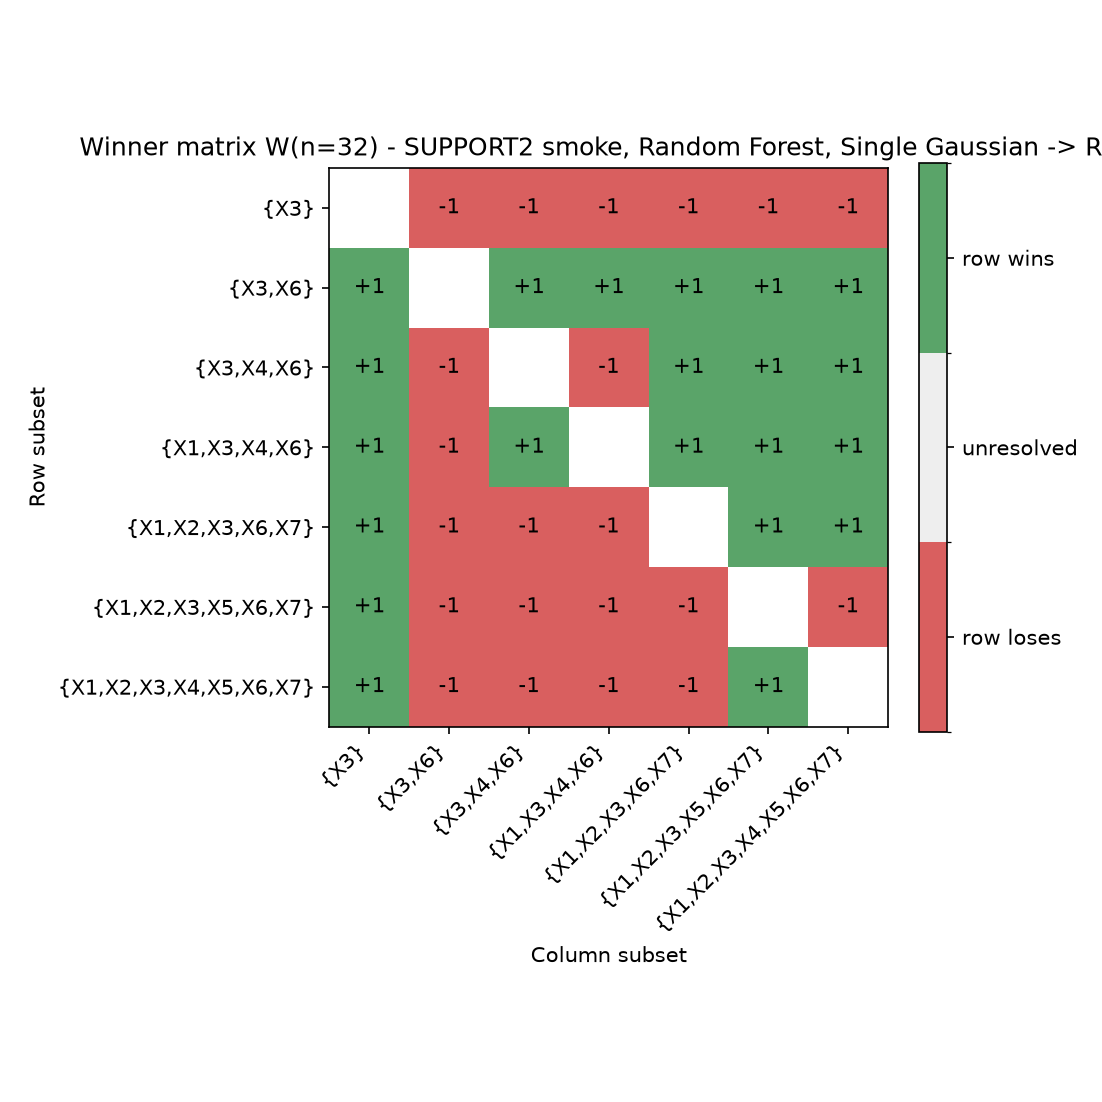
\includegraphics[width=0.46\textwidth]{figures/wr_matrices/support2_smoke/winner_matrix_single_gaussian_to_real_n32.png}
  \hfill
  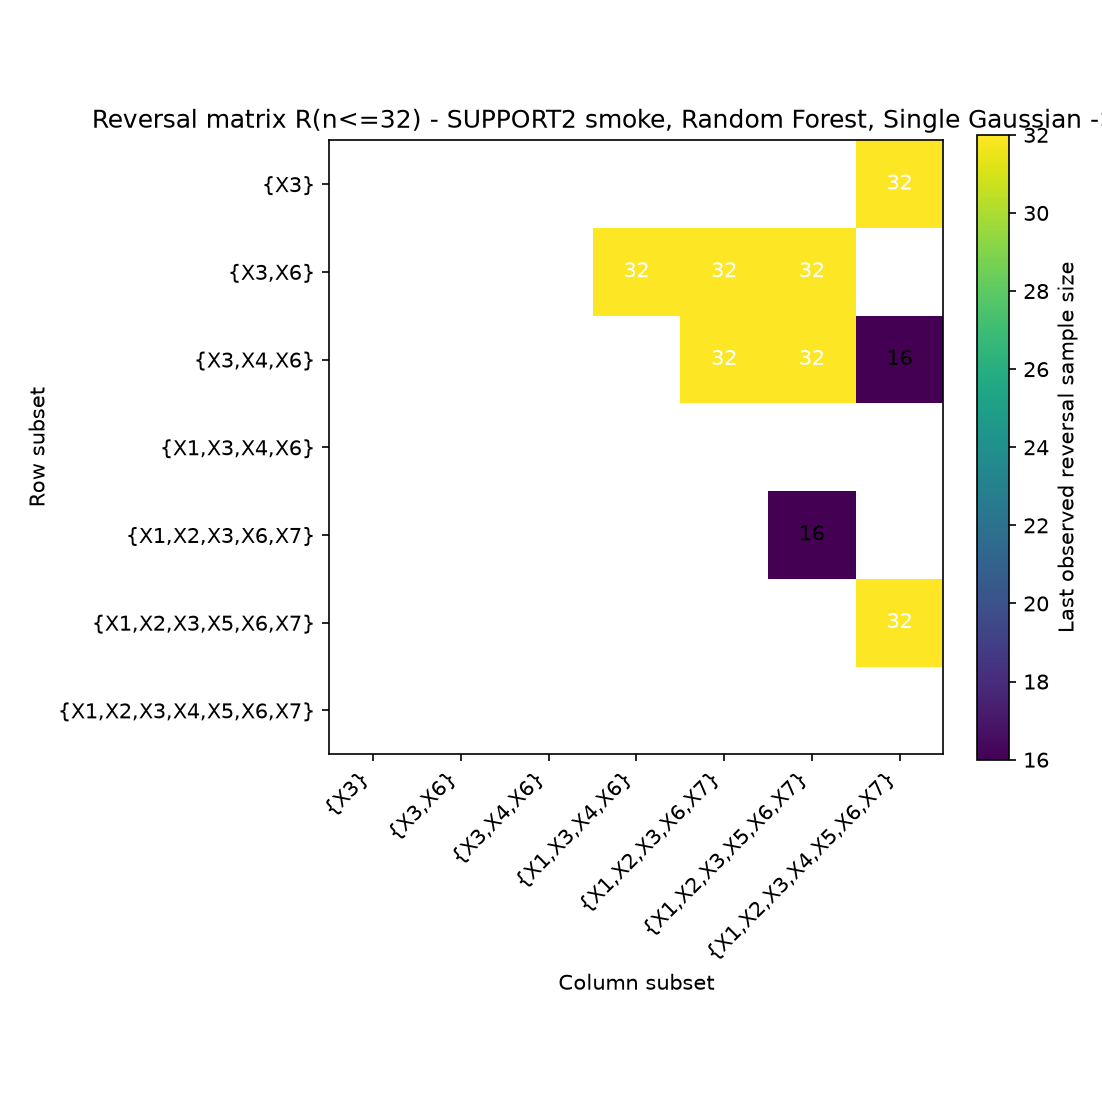
\includegraphics[width=0.46\textwidth]{figures/wr_matrices/support2_smoke/reversal_matrix_single_gaussian_to_real_n32.png}
  \sourcebelow{recomputado diretamente dos resultados persistidos da execução \textit{smoke} do SUPPORT2; mesmas matrizes já apresentadas na Figura~\ref{fig:wr-matrices-support2} do Capítulo~6, reproduzidas aqui em contexto de resultados}
\end{figure}

\subsection{Comparação do Random Forest com os demais classificadores}

Sob os indicadores herdados $\rankrho$ e $\AW$, o Random Forest do cenário 000008 não se destacou por um valor de similaridade de $\NstarHistorical$ mais alto do que os demais classificadores do SUPPORT2 --- essa comparação, central nas versões anteriores deste relatório, dependia inteiramente do objeto retirado do arcabouço ativo e não pode ser refeita sob o esquema atual sem os dados brutos das execuções \textit{full} correspondentes (Seção~\ref{sec:resultados-guia}). O que permanece observável é que o Random Forest combinou o menor desempenho preditivo absoluto entre os classificadores estudados (perda próxima do referencial majoritário) com valores de $\rankrho$ e $\AW$ comparáveis aos dos classificadores lineares no mesmo cenário --- reforçando, já nos indicadores herdados, que desempenho absoluto e preservação da ordenação/relações de vencedor são propriedades distintas. A relação desse classificador com a existência e o regime amostral das inversões, especificamente, só pôde ser reexaminada na escala reduzida da execução \textit{smoke} (Seção~\ref{sec:support2-rf}).

Esse resultado não pode ser generalizado para Occupancy e Air Quality, pois o Random Forest não foi executado nesses datasets. A execução foi aproximadamente três a cinco vezes mais lenta que as simulações com classificadores mais simples, inviabilizando a repetição completa dentro do prazo do trabalho. O resultado é, portanto, evidência de uma interação específica entre SUPPORT2, Random Forest e os geradores avaliados.

\section{Síntese dos cenários}

A Tabela~\ref{tab:cross-synthesis} resume os padrões mais informativos observáveis nos indicadores disponíveis nesta revisão. Não existe um gerador universalmente superior. O classificador é decisivo: Gaussian Naive Bayes no Air Quality apresentou a preservação mais alta de ordenação e relações de vencedor do estudo, enquanto o Random Forest no SUPPORT2 combinou baixa qualidade preditiva absoluta com preservação de ordenação e relações de vencedor comparável à dos classificadores lineares --- e, no exemplo em escala reduzida da Seção~\ref{sec:support2-rf}, com um perfil particular de $\AR$ mais baixo e $\SR$ mais alto do que o SVM linear.

\begin{table}[H]
  \centering
  \caption{Síntese qualitativa dos resultados experimentais}
  \label{tab:cross-synthesis}
  \begin{tabularx}{\textwidth}{p{2.7cm}p{3.0cm}X}
    \toprule
    Dataset & Configuração destacada & Resultado central \\
    \midrule
    Occupancy & SVM, Gaussiana única & Geometria visualmente pobre, mas $\rankrho$ e $\AW$ superiores aos do GMM em $n=512$ (valores herdados). \\
    Occupancy & GNB, GMM & $\rankrho$ e $\AW$ quase perfeitos (valores herdados); $\AR$/$\SR$ indisponíveis nesta revisão. \\
    Air Quality & GNB, ambos os braços sintéticos & Preservação quase integral de $\rankrho$ e $\AW$ (valores herdados); $\AR$/$\SR$ indisponíveis nesta revisão. \\
    SUPPORT2 & SVM e regressão logística & $\rankrho$ e $\AW$ altos em $n=512$ (valores herdados); $\AR$/$\SR$ indisponíveis nesta revisão. \\
    SUPPORT2 & Random Forest (\textit{full}, $n=512$) & Perda próxima ao referencial majoritário; $\rankrho$/$\AW$ herdados comparáveis aos classificadores lineares; $\AR$/$\SR$ indisponíveis nesta revisão. \\
    SUPPORT2 & Random Forest e SVM (\textit{smoke}, $n\leq32$) & Único exemplo com $\AR$ e $\SR$ recalculados pelo código atual: RF preserva pior a existência das inversões, mas melhor seu regime amostral, do que o SVM linear. \\
    \bottomrule
  \end{tabularx}
  \sourcebelow{elaboração própria}
\end{table}

Em conjunto, os resultados disponíveis nesta revisão respondem afirmativamente, mas de forma condicionada, à pergunta central, no que se refere à ordenação global e às relações efetivas de vencedor: os perfis de cooperação preditiva que emergem do treinamento de classificadores com amostras sintéticas, produzidas por geradores ajustados aos dados reais de treinamento, podem reproduzir componentes importantes do perfil que emerge do treinamento com amostras reais. Essa preservação não é uniforme, não coincide obrigatoriamente com semelhança visual e não pode ser inferida apenas da perda absoluta. Quanto à existência e ao regime amostral das inversões --- as duas questões mais finas do perfil ---, esta revisão só pôde oferecer evidência numérica corrente em escala reduzida (SUPPORT2 \textit{smoke}); a caracterização completa dessas duas dimensões nos três datasets em escala publicada permanece pendente de regeneração dos dados brutos correspondentes, conforme detalhado no Apêndice~B.
